%**************************************%
%* Generated from MathBook XML source *%
%*    on 2016-01-19T11:51:14-05:00    *%
%*                                    *%
%*   http://mathbook.pugetsound.edu   *%
%*                                    *%
%**************************************%
\documentclass[10pt,]{book}
%% Load geometry package to allow page margin adjustments
\usepackage{geometry}
\geometry{letterpaper,total={5.0in,9.0in}}
%% Custom Preamble Entries, early (use latex.preamble.early)
%% Inline math delimiters, \(, \), made robust with next package
\usepackage{fixltx2e}
%% Page Layout Adjustments (latex.geometry)
%% For unicode character support, use the "xelatex" executable
%% If never using xelatex, the next three lines can be removed
\usepackage{ifxetex}
\ifxetex\usepackage{xltxtra}\fi
%% Symbols, align environment, bracket-matrix
\usepackage{amsmath}
\usepackage{amssymb}
%% allow more columns to a matrix
%% can make this even bigger by overiding with  latex.preamble.late  processing option
\setcounter{MaxMatrixCols}{30}
%% XML, MathJax Conflict Macros
%% Two nonstandard macros that MathJax supports automatically
%% so we always define them in order to allow their use and
%% maintain source level compatibility
%% This avoids using two XML entities in source mathematics
\newcommand{\lt}{<}
\newcommand{\gt}{>}
%% Semantic Macros
%% To preserve meaning in a LaTeX file
%% Only defined here if required in this document
%% Subdivision Numbering, Chapters, Sections, Subsections, etc
%% Subdivision numbers may be turned off at some level ("depth")
%% A section *always* has depth 1, contrary to us counting from the document root
%% The latex default is 3.  If a larger number is present here, then
%% removing this command may make some cross-references ambiguous
%% The precursor variable $numbering-maxlevel is checked for consistency in the common XSL file
\setcounter{secnumdepth}{3}
%% Environments with amsthm package
%% Theorem-like enviroments in "plain" style, with or without proof
\usepackage{amsthm}
\theoremstyle{plain}
%% Numbering for Theorems, Conjectures, Examples, Figures, etc
%% Controlled by  numbering.theorems.level  processing parameter
%% Always need a theorem environment to set base numbering scheme
%% even if document has no theorems (but has other environments)
\newtheorem{theorem}{Theorem}[section]
%% Only variants actually used in document appear here
%% Numbering: all theorem-like numbered consecutively
%% i.e. Corollary 4.3 follows Theorem 4.2
\newtheorem{algorithm}[theorem]{Algorithm}
%% Definition-like environments, normal text
%% Numbering for definition, examples is in sync with theorems, etc
%% also for free-form exercises, not in exercise sections
\theoremstyle{definition}
\newtheorem{definition}[theorem]{Definition}
\newtheorem{example}[theorem]{Example}
\newtheorem{exercise}[theorem]{Exercise}
%% Localize LaTeX supplied names (possibly none)
\renewcommand*{\proofname}{Proof}
\renewcommand*{\chaptername}{Chapter}
%% Figures, Tables, Listings, Floats
%% The [H]ere option of the float package fixes floats in-place,
%% in deference to web usage, where floats are totally irrelevant
%% We re/define the figure, table and listing environments, if used
%%   1) New mbxfigure and/or mbxtable environments are defined with float package
%%   2) Standard LaTeX environments redefined to use new environments
%%   3) Standard LaTeX environments redefined to step theorem counter
%%   4) Counter for new enviroments is set to the theorem counter before caption
%% You can remove all this figure/table setup, to restore standard LaTeX behavior
%% HOWEVER, numbering of figures/tables AND theorems/examples/remarks, etc
%% WILL ALL de-synchronize with the numbering in the HTML version
%% You can remove the [H] argument of the \newfloat command, to allow flotation and 
%% preserve numbering, BUT the numbering may then appear "out-of-order"
\usepackage{float}
\usepackage[bf]{caption} % http://tex.stackexchange.com/questions/95631/defining-a-new-type-of-floating-environment 
\usepackage{newfloat}
% Figure environment setup so that it no longer floats
\SetupFloatingEnvironment{figure}{fileext=lof,placement={H},within=section,name=Figure}
% figures have the same number as theorems: http://tex.stackexchange.com/questions/16195/how-to-make-equations-figures-and-theorems-use-the-same-numbering-scheme 
\makeatletter
\let\c@figure\c@theorem
\makeatother
% Table environment setup so that it no longer floats
\SetupFloatingEnvironment{table}{fileext=lot,placement={H},within=section,name=Table}
% tables have the same number as theorems: http://tex.stackexchange.com/questions/16195/how-to-make-equations-figures-and-theorems-use-the-same-numbering-scheme 
\makeatletter
\let\c@table\c@theorem
\makeatother
%% Raster graphics inclusion, wrapped figures in paragraphs
\usepackage{graphicx}
%% Colors for Sage boxes and author tools (red hilites)
\usepackage[usenames,dvipsnames,svgnames,table]{xcolor}
%% New typewriter font if  c, sage, program, console, pre  tags present
%% If only  email, url  tags, no change from default
%% Needs a bit of scaling down to match text
\usepackage[scaled=.95]{sourcecodepro}
%% Program listing support, for inline code, Sage code
\usepackage{listings}
%% We define the listings font style to be the default "ttfamily"
%% To fix hyphens/dashes rendered in PDF as fancy minus signs by listing
%% http://tex.stackexchange.com/questions/33185/listings-package-changes-hyphens-to-minus-signs
\makeatletter
\lst@CCPutMacro\lst@ProcessOther {"2D}{\lst@ttfamily{-{}}{-{}}}
\@empty\z@\@empty
\makeatother
%% End of generic listing adjustments
%% Sage's blue is 50%, we go way lighter (blue!05 would work)
\definecolor{sageblue}{rgb}{0.95,0.95,1}
%% Sage input, listings package: Python syntax, boxed, colored, line breaking
%% Indent from left margin, flush at right margin
\lstdefinestyle{sageinput}{language=Python,breaklines=true,breakatwhitespace=true,basicstyle=\small\ttfamily,columns=fixed,frame=single,backgroundcolor=\color{sageblue},xleftmargin=4ex}
%% Sage output, similar, but not boxed, not colored
\lstdefinestyle{sageoutput}{language=Python,breaklines=true,breakatwhitespace=true,basicstyle=\small\ttfamily,columns=fixed,xleftmargin=4ex}
%% Multiple column, column-major lists
\usepackage{multicol}
%% More flexible list management, esp. for references and exercises
%% But also for specifying labels (ie custom order) on nested lists
\usepackage{enumitem}
%% Lists of exercises in their own section, maximum depth 4
\newlist{exerciselist}{description}{4}
\setlist[exerciselist]{leftmargin=0pt,itemsep=1.0ex,topsep=1.0ex,partopsep=0pt,parsep=0pt}
%% Indented groups of exercises within an exercise section, maximum depth 4
\newlist{exercisegroup}{description}{4}
\setlist[exercisegroup]{leftmargin=2em,labelindent=2em,itemsep=1.0ex,topsep=1.0ex,partopsep=0pt,parsep=0pt}
%% Package for tables spanning several pages
\usepackage{longtable}
%% hyperref driver does not need to be specified
\usepackage{hyperref}
%% Hyperlinking active in PDFs, all links solid and blue
\hypersetup{colorlinks=true,linkcolor=blue,citecolor=blue,filecolor=blue,urlcolor=blue}
\hypersetup{pdftitle={Applied Discrete Structures}}
%% If you manually remove hyperref, leave in this next command
\providecommand\phantomsection{}
%% Use upright quotes rather than LaTeX's curly quotes
%% If custom font substitutions follow, this might be ineffective
%% If fonts lack upright quotes, the textcomp package is employed
\usepackage{upquote}
%% Graphics Preamble Entries
%% extpfeil package for certain extensible arrows,
%% as also provided by MathJax extension of the same name
%% NB: this package loads mtools, which loads calc, which redefines
%%     \setlength, so it can be removed if it seems to be in the 
%%     way and your math does not use:
%%     
%%     \xtwoheadrightarrow, \xtwoheadleftarrow, \xmapsto, \xlongequal, \xtofrom
%%     
%%     we have had to be extra careful with variable thickness
%%     lines in tables, and so also load this package late
\usepackage{extpfeil}
%% Custom Preamble Entries, late (use latex.preamble.late)
%% Convenience macros
\newcommand{\identity}{\mathrm{id}}
\newcommand{\notdivide}{{\not{\mid}}}
\newcommand{\notsubset}{\not\subset}
\newcommand{\lcm}{\operatorname{lcm}}
\newcommand{\gf}{\operatorname{GF}}
\newcommand{\inn}{\operatorname{Inn}}
\newcommand{\aut}{\operatorname{Aut}}
\newcommand{\Hom}{\operatorname{Hom}}
\newcommand{\cis}{\operatorname{cis}}
\newcommand{\chr}{\operatorname{char}}
\newcommand{\Null}{\operatorname{Null}}
%% Title page information for book
\title{Applied Discrete Structures}
\author{Al Doerr\\
Department of Mathematical Sciences\\
University of Massachusetts Lowell\\
\href{mailto:}{\nolinkurl{}}
\and
Ken Levasseur\\
Department of Mathematical Sciences\\
University of Massachusetts Lowell\\
\href{mailto:kenneth_levasseur@uml.edu}{\nolinkurl{kenneth_levasseur@uml.edu}}
}
\date{January 4, 2016}
\begin{document}
\frontmatter
%% begin: half-title
\thispagestyle{empty}
{\centering
\vspace*{0.28\textheight}
{\Huge Applied Discrete Structures}\\}
\clearpage
%% end:   half-title
%% begin: adcard
\thispagestyle{empty}
\null%
\clearpage
%% end:   adcard
%% begin: title page
%% Inspired by Peter Wilson's "titleDB" in "titlepages" CTAN package
\thispagestyle{empty}
{\centering
\vspace*{0.14\textheight}
{\Huge Applied Discrete Structures}\\[3\baselineskip]
{\Large Al Doerr}\\[0.5\baselineskip]
{\Large University of Massachusetts Lowell}\\[3\baselineskip]
{\Large Ken Levasseur}\\[0.5\baselineskip]
{\Large University of Massachusetts Lowell}\\[3\baselineskip]
{\Large January 4, 2016}\\}
\clearpage
%% end:   title page
%% begin: copyright-page
\thispagestyle{empty}
\vspace*{\stretch{2}}
\noindent\copyright\ 2011\textendash{}2016\quad{}Al Doerr, Ken Levasseur\\[0.5\baselineskip]
\emph{Applied Discrete Structures} by Alan Doerr and Kenneth Levasseur is licensed under a Creative Commons Attribution-NonCommercial-ShareAlike 3.0 United States License. You are free to:
			\leavevmode%
\begin{itemize}[label=\textbullet]
\item{}Share — copy and redistribute the material in any medium or format\item{}Adapt — remix, transform, and build upon the material\end{itemize}

			You may not use the material for commercial purposes.  The licensor cannot revoke these freedoms as long as you follow the license terms.%

			\par
\vspace*{\stretch{1}}
\null\clearpage
%% end:   copyright-page
%% begin: acknowledgement
\chapter*{Acknowledgements}\label{acknowledgement-1}
\addcontentsline{toc}{chapter}{Acknowledgements}
We would like to acknowledge the following reviewers for their helpful comments and suggestions. %
\leavevmode%
\begin{itemize}[label=\textbullet]
\item{}Tibor Beke, UMass Lowell\item{}Alex DeCourcy, UMass Lowell\item{}Ravi Montenegro, UMass Lowell\item{}Jim Propp, UMass Lowell\item{}Students at Luzurne County Community College (PA)\end{itemize}
\par
I would  like to thank Rob Beezer for his guidance and work on MathBook XML as we start this project.%
%% end:   acknowledgement
%% begin: preface
\chapter*{Preface}\label{preface-1}
\addcontentsline{toc}{chapter}{Preface}
This version of \emph{Applied Discrete Structures} is being developed using \emph{Mathbook XML}, A lightweight XML application for authors of scientific articles, textbooks and monographs initiated by Rob Beezer, U. of Puget Sound.  %
\par
\emph{Status:}  The first  two chapters have been converted by hand to Mathbook XML as a learning process.  Plans are now to explore ways to convert remaining Mathematica Notebooks in a more systematic way.%
\par
Sage (\href{http://sagemath.org}{sagemath.org}) is a free, open source, software system for advanced mathematics.  Sage can be used either on your own computer, a local server, or on SageMathCloud (\href{https://cloud.sagemath.com}{https://cloud.sagemath.com}). %
\begin{quote}
			Ken Levasseur \newline{}
			Lowell MA
		\end{quote}%% end:   preface
%% begin: table of contents
\setcounter{tocdepth}{1}
\renewcommand*\contentsname{Contents}
\tableofcontents
%% end:   table of contents
\mainmatter
\typeout{************************************************}
\typeout{Chapter 1 Set Theory I}
\typeout{************************************************}
\chapter[Set Theory I]{Set Theory I}\label{chapter-1}
\typeout{************************************************}
\typeout{Introduction  Goals for Chapter 1}
\typeout{************************************************}
\section*{Goals for Chapter 1}
\typeout{************************************************}
\typeout{Section 1.1 Set Notation and Relations }
\typeout{************************************************}
\section[Set Notation and Relations ]{Set Notation and Relations }\label{Set-Notation-and-Relations}
\typeout{************************************************}
\typeout{Subsection 1.1.1 The notion of a set}
\typeout{************************************************}
\subsection[The notion of a set]{The notion of a set}\label{subsection-1}
The term set is intuitively understood by most people to mean a collection of objects that are called elements (of the set). This concept is the
starting point on which we will build more complex ideas, much as in-geometry where the concepts of point and line are left undefined. 
Because a set is such a simple notion, you may be surprised to learn that it is one of the most difficult concepts for mathematicians to define to
their own liking. For example, the description above is not a proper definition because it requires the definition of a collection. (How would you
define ``collection''?) Even deeper problems arise when you consider the possibility that a set could contain itself. Although these problems
are of real concern to some mathematicians, they will not be of any concern to us. 
Our first concern will be how to describe a set; that is, how do we most conveniently describe a set and the elements that are in it? If we are going to discuss a set for any length of time, we usually give it a name in the form of a capital letter (or occasionally some other symbol). In discussing set \( A\), if \( x\) is an element of \( A\), then we will write \(x \in  A\). On the other hand, if \( x\) is not an element
of \( A\), we write \(x \notin  A\). The most convenient way of describing the elements of a set will vary depending on the specific set. %
\par
\emph{ Enumeration.} When the elements of a set are enumerated (or listed) it is traditional to enclose them in braces. For example, the
set of binary digits is\(\{0, 1\}\) and the set of decimal digits is \(\{0, 1, 2, 3, 4, 5, 6, 7, 8, 9\}\). The choice of a name for these sets would
be arbitrary; but it would be ``logical'' to call them \( B\) and \( D\) , respectively. The choice of a set name is much like the
choice of an identifier name in programming. Some large sets can be enumerated without actually listing all the elements. For example, the letters
of the alphabet and the integers from 1 to 100 could be described as 
\(A = \{a, b, c,\ldots , x, y, z\}\), and \(G = \{1, 2, \ldots  , 99, 100\}\). 
The three consecutive ``dots'' are called an ellipsis. We use them when it is clear what elements are included but not listed. An ellipsis is
used in two other situations. To enumerate the positive integers, we would write \(\{1, 2, 3,\ldots  \}\), indicating that the list goes on infinitely.
If we want to list a more general set such as the integers between 1 and \( n\), where \( n\) is some undetermined positive integer, we
might write \(\{1,\ldots ,n\}\).
%
\par
\emph{ Standard Symbols}. Frequently used sets are usually given symbols that are reserved for them alone. For example, since we will be
referring to the positive integers throughout this book, we will use the symbol \(\mathbb{P}\) instead of writing \(\{1, 2, 3, \ldots \}\). A few
of the other sets of numbers that we will use frequently are: 
\leavevmode%
\begin{itemize}[label=\textbullet]
\item{}\(\mathbb{N}\) for the natural numbers, \(\{0, 1, 2, 3, \ldots \}\)\item{}\(\mathbb{Z}\) for the integers, \(\{\ldots , -3, -2, -1, 0, 1, 2, 3,\ldots \}\)\item{}\(\mathbb{Q}\) for the rational numbers\item{}\(\mathbb{R}\) for the real numbers\item{}\(\mathbb{C}\) for the complex numbers\end{itemize}

%
\par
\emph{ Set-Builder Notation}. Another way of describing sets is to use set-builder notation. For example, we could define the rational numbers as \(\mathbb{Q}=\{a/b : a, b \in  \mathbb{Z}, b\neq 0\}\).  Note that in the set-builder description for the rational numbers: 
\leavevmode%
\begin{itemize}[label=\textbullet]
\item{} \(a/b\) indicates that a typical element of the set is a ``fraction.'' \item{} The colon is read ``such that'' or ``where,'' and is used interchangeably with a vertical line, \(\mid\). 
 \item{} \(a, b\in \mathbb{Z}\) is an abbreviated way of saying \(a\) and \(b\) are integers. 
 \item{} All commas in mathematics are read as ``and.'' 
\end{itemize}

The important fact to keep in mind in set notation, or in any mathematical notation, is that it is meant to be a help, not a hindrance. We hope that notation will assist us in a more complete understanding of the collection of objects under consideration and will enable us to describe it in a concise manner. However, brevity of notation is not the aim of sets. If you prefer to write \(a\in \mathbb{Z}\) and \(b\in \mathbb{Z}\) instead of \(a, b\in \mathbb{Z}\), you should do so. Also, there are frequently many different, and equally good, ways of describing sets. For example, \(\left\{x\in
\mathbb{R}\left| x^{2 }-5x+6\right.=0\right\}\) and \(\left\{x \left| x\in \mathbb{R}: x^{2 }-5x+6\right.=0\right\}\) both describe the solution set \(\{2, 3\}\). 
%
\par
A proper definition of the real numbers is beyond the scope of this text. It is sufficient to think of the real numbers as the set of points on a
number line. The complex numbers can be defined using set-builder notation as \(\mathbb{C} = \{a + b i:a, b \in \mathbb{R}\}\), where \(i^2 = -1\).  %
\par
In the following definition we will leave the word ``finite'' undefined.   
%
\begin{definition}[ Finite Set.]\label{finite-set}
A set is a finite set if it has a finite number of elements. Any set that is not finite is an infinite set.
	\end{definition}
\begin{definition}[ Cardinality.]\label{cardinality.}
Let A be a finite set. The number of different elements in A is called its cardinality.
\end{definition}
\label{notation-1}
\par
As we will see later, there are different infinite cardinalities. We can't make this distinction now, so we will restrict cardinality to finite sets
until later.%
\typeout{************************************************}
\typeout{Subsection 1.1.2 Subsets}
\typeout{************************************************}
\subsection[Subsets]{Subsets}\label{subsection-2}
\begin{definition}[ Subset.]\label{subset.}
 Let \(A\) and \(B\) be sets. We say that \(A\) is a subset of \(b\)  if and only if every element of \(A\) is an element of \(b\). 
\end{definition}
\label{notation-2}
\begin{example}[ Some Subsets ]\label{Some_Subsets}
\leavevmode%
\begin{enumerate}
\item\hypertarget{li-17}{} If \(A = \{3, 5, 8\}\) and \(B = \{5, 8, 3, 2, 6\}\), then \(A\subseteq B\). \item\hypertarget{li-18}{}  \(\mathbb{N}\subseteq \mathbb{Z}\subseteq \mathbb{Q}\subseteq \mathbb{R}\subseteq \mathbb{C}\) 
 \item\hypertarget{li-19}{}If \(A = \{3, 5, 8\}\) and \(B = \{5, 3, 8\}\), then \(A \subseteq  B\) and \(B \subseteq  A\). \end{enumerate}

%
\end{example}
\begin{definition}[ Set Equality. ]\label{set_equality}
Let \(A\) and \(B\) be sets. We say that \(A\) is equal to \(B\) (notation \(A = B\)) if and only if every element of
A is an element of B and conversely every element of B is an element of A; that is, \(A \subseteq  B\) and \(B \subseteq  A\). 
\end{definition}
\begin{example}[ Examples illustrating set equality]\label{set_equality_examples}
\leavevmode%
\begin{multicols}{1}
\begin{enumerate}
\item\hypertarget{li-20}{}In the previous example, \(A = B\). Note that the ordering of the elements is unimportant. \item\hypertarget{li-21}{}The number of times that an element appears in an enumeration doesn't affect a set. For example, if \(A = \{1, 5, 3, 5\}\) and \(B = \{1, 5, 3\}\), then \(A = B\).  Warning to readers of other texts: Some books introduce the concept of a multiset, in which the number of occurrences of an element matters.\end{enumerate}
\end{multicols}

%
\end{example}
A few comments are in order about the expression ``if and only if'' as used in our definitions. This expression means ``is equivalent to saying,''
or more exactly, that the word (or concept) being defined can at any time be replaced by the defining expression. Conversely, the expression that
defines the word (or concept) can be replaced by the word. %
\par
Occasionally there is need to discuss the set that contains no elements, namely the empty set, which is denoted by \(\emptyset\).
This set is also called the null set.%
\par
It is clear, we hope, from the definition of a subset, that given any set \( A\) we have \(A\subseteq A\) and \(\emptyset \subseteq A\). Both
\(\emptyset\) and \( A\) are called \emph{improper subsets }of \(A\). If \(B \subseteq  A\), \(B\neq \emptyset\), and \(B\neq A\),
then \(B\) is called a \emph{ proper subset} of \(A\).%
\typeout{************************************************}
\typeout{Exercises 1.1.3 Exercises for Section 1.1 }
\typeout{************************************************}
\subsection[Exercises for Section 1.1 ]{Exercises for Section 1.1 }\label{exercises-1}
\hypertarget{exercisegroup-1}{}\typeout{************************************************}
\typeout{Introduction  }
\typeout{************************************************}
A Exercises%
\begin{exercisegroup}
\item[1.]\hypertarget{exercise-1}{}
 List four elements of each of the following sets:
\leavevmode%
\begin{multicols}{1}
\begin{enumerate}[label=(\alph*)]
\item\hypertarget{li-22}{} \(\{k \in  \mathbb{P} \mid {k - 1} \textrm{ is a multiple of 7}\}\) \item\hypertarget{li-23}{} \(\{x \mid x \textrm{ is a fruit and its skin is normally eaten }\}\)\item\hypertarget{li-24}{}\(\{x \in \mathbb{Q}\mid x\in \mathbb{Z}\}\)\item\hypertarget{li-25}{} \(\{2n \mid n \in \mathbb{Z}, n < 0 \}\)\item\hypertarget{li-26}{} \(\{s \mid s = 1 + 2 + \cdots  + n, n \in \mathbb{P}\}\)\end{enumerate}
\end{multicols}
\par\smallskip
\item[2.]\hypertarget{exercise-2}{}  List all elements of the following sets:
\leavevmode%
\begin{multicols}{1}
\begin{enumerate}[label=(\alph*)]
\item\hypertarget{li-27}{} \(\{\frac{1}{n} \mid n \in \{3,4,5,6\}\}\) 
  \item\hypertarget{li-28}{}  \(\{\alpha \in  \textrm{the alphabet} \mid  \textrm{\alpha precedes F\ }\) 
  \item\hypertarget{li-29}{} \(\{-k \mid k \in \mathbb{P}\}\) 
  \item\hypertarget{li-30}{} \(\{n^2 \mid  n = -2, -1, 0, 1, 2\}\) 
  \item\hypertarget{li-31}{} \(\{n \in  \mathbb{P} \mid n \textrm{is a  factor of  24 }\}\) 
  \end{enumerate}
\end{multicols}
\par\smallskip
\item[3.]\hypertarget{exercise-3}{}  Describe the following sets using set-builder notation. 
\leavevmode%
\begin{multicols}{1}
\begin{enumerate}[label=(\alph*)]
\item\hypertarget{li-32}{} \(\{ 5, 7, 9, \dots , 77, 79\}\) \item\hypertarget{li-33}{}the rational numbers that are strictly between \(-1\) and \(1\) \item\hypertarget{li-34}{} the even integers\item\hypertarget{li-35}{} \(\{-18, -9,0,9, 18,27, \dots \}\) \end{enumerate}
\end{multicols}
\par\smallskip
\item[4.]\hypertarget{exercise-4}{}  Use set-builder notation to describe the following sets: 
\leavevmode%
\begin{multicols}{1}
\begin{enumerate}[label=(\alph*)]
\item\hypertarget{li-36}{}\(\{1, 2, 3, 4, 5, 6, 7\}\) \item\hypertarget{li-37}{} \(\{1, 10, 100, 1000, 10000\}\)  \item\hypertarget{li-38}{} \(\{1, 1/2, 1/3, 1/4, 1/5, . . .\}\) \item\hypertarget{li-39}{}  \(\{0\}\)\end{enumerate}
\end{multicols}
\par\smallskip
\item[5.]\hypertarget{exercise-5}{}  Let \(A = \{0, 2, 3\}\), \(B = \{2, 3\}\), and \(C = \{1, 5, 9\}\). Determine which of the following statements are true. Give reasons for
your answers. 
\leavevmode%
\begin{multicols}{2}
\begin{enumerate}[label=(\alph*)]
\item\hypertarget{li-40}{}\(3 \in  A\)\item\hypertarget{li-41}{}\(\{3\} \in  A\) \item\hypertarget{li-42}{}\(\{3\} \subseteq A\)\item\hypertarget{li-43}{} \(B\subseteq A\)\item\hypertarget{li-44}{} \(A\subseteq B\)\item\hypertarget{li-45}{}\(\emptyset \subseteq C\) \item\hypertarget{li-46}{} \(\emptyset \in A\)\item\hypertarget{li-47}{} \(A\subseteq A\)\end{enumerate}
\end{multicols}
\par\smallskip
\end{exercisegroup}
\par\smallskip\noindent
\hypertarget{exercisegroup-2}{}\typeout{************************************************}
\typeout{Introduction  }
\typeout{************************************************}
C Exercises%
\begin{exercisegroup}
\item[6.]\hypertarget{exercise-6}{}  One reason that we left the definition of a set vague is Russell's Paradox. Many mathematics and logic books contain an account of this paradox.
Two references are Stoll and Quine. Find one such reference and read it.  
\par\smallskip
\end{exercisegroup}
\par\smallskip\noindent
\typeout{************************************************}
\typeout{Section 1.2 Basic Set Operations  }
\typeout{************************************************}
\section[Basic Set Operations  ]{Basic Set Operations  }\label{Basic_Set_Operations}
\typeout{************************************************}
\typeout{Subsection 1.2.1 Definitions}
\typeout{************************************************}
\subsection[Definitions]{Definitions}\label{subsection-3}
\begin{definition}[ Intersection]\label{intersection}
 Let \(A\) and \(B\) be sets. The intersection of \(A\) and \(B\) (denoted by \(A \cap  B\)) is the set of all elements
that are in both \(A\) and \(B\). That is, \(A \cap  B = \{x:x \in  A \textrm{ and } x \in  B)\). 
\end{definition}
\label{notation-3}
\begin{example}[Some Intersections]\label{some_intersections}
\leavevmode%
\begin{itemize}[label=\textbullet]
\item{} Let \(A = \{1, 3, 8\}\) and \(B = \{-9, 22, 3\}\). Then \(A \cap  B = \{3\}\).\item{}Solving a system of simultaneous equations such as \(x + y = 7\) and \(x - y = 3\) can be viewed as an intersection. Let \(A = \{(x,y): x + y = 7, x,y \in  \mathbb{R}\}\) and \(B = \{(x,y): x - y - 3, x,y\in  \mathbb{R}\}\). These two sets are lines in the plane and their intersection,
\(A \cap  B = \{(5, 2)\}\), is the solution to the system. \item{} \(\mathbb{Z}\cap \mathbb{Q}=\mathbb{Z}\). \item{}If \(A = \{3, 5, 9\}\) and \(B = \{-5, 8\}\), then \(A\cap  B =\emptyset\). \end{itemize}
%
\end{example}
\begin{definition}[ Disjoint Sets.]\label{disjoint-sets.}
Two sete are disjoint if they have no elements in common (as in Example 1.2.1 d). That is, \(A\) and \(B\) are disjoint if \(A \cap  B = \emptyset\).
\end{definition}
\begin{definition}[ Union.]\label{union.}
 Let \(A\) and \(B\) be sets. The union of \(A\) and \(B\) (denoted by \(A \cup  B\)) is the set of all elements that are
in \(A\) or in \(B\) or in both A and B. That is, \(A\cup B= \{x:x \in  A\textrm{ or } x\in  B\}\). 
It is important to note in the set-builder notation for \(A\cup B\), the word ``or'' is used in the inclusive sense; it includes the case where
\( x\) is in both \(A\) and \(B\).
\end{definition}
\label{notation-4}
\begin{example}[Some Unions]\label{some_unions}
\leavevmode%
\begin{itemize}[label=\textbullet]
\item{} If \(A = \{2, 5, 8\}\) and  \(B = \{7, 5, 22\}\), then \(A \cup  B = \{2, 5, 8, 7, 22\}\). \item{} \(\mathbb{Z}\cup \mathbb{Q}=\mathbb{Q}.\) \item{} \(A \cup \emptyset  = A\) for any set \(A\).\end{itemize}
%
\end{example}
Frequently, when doing mathematics, we need to establish a universe or set of elements under discussion. For example, the set \(A = \{x : 81x^4 -16 = 0 \}\) contains different elements depending on what kinds of numbers we allow ourselves to use in solving the equation \(81 x^4 -16 = 0\). This set of numbers would be our universe. For example, if the universe is the integers, then \(A\) is empty. If our universe is the
rational numbers, then \( A\) is \(\{2/3, -2/3\}\) and if the universe is the complex numbers, then A is \(\{2/3, -2/3, 2i/3, - 2i/3\}\).
%
\begin{definition}[ Universe.]\label{universe.}
 The universe, or universal set, is the set of all elements under discussion for possible membership
in a set. We normally reserve the letter \( U\) for a universe in general discussions.   
\end{definition}
\typeout{************************************************}
\typeout{Subsection 1.2.2 Set Operations and their Venn Diagams }
\typeout{************************************************}
\subsection[Set Operations and their Venn Diagams ]{Set Operations and their Venn Diagams }\label{subsection-4}
When working with sets, as in other branches of mathematics, it is often quite useful to be able to draw a picture or diagram of the situation under consideration. A diagram of a set is called a Venn diagram. The universal set U is represented by the interior of a rectangle and the sets by disks inside the rectangle.%
\begin{example}[Venn Diagram Examples]\label{venn_diagram_examples}
(a) \(A \cap  B\) is illustrated in the following figure by shading the appropriate region. 
           \leavevmode%
\begin{figure}
\centering
\IfFileExists{images/sageplot-venn-intersection.pdf}%
{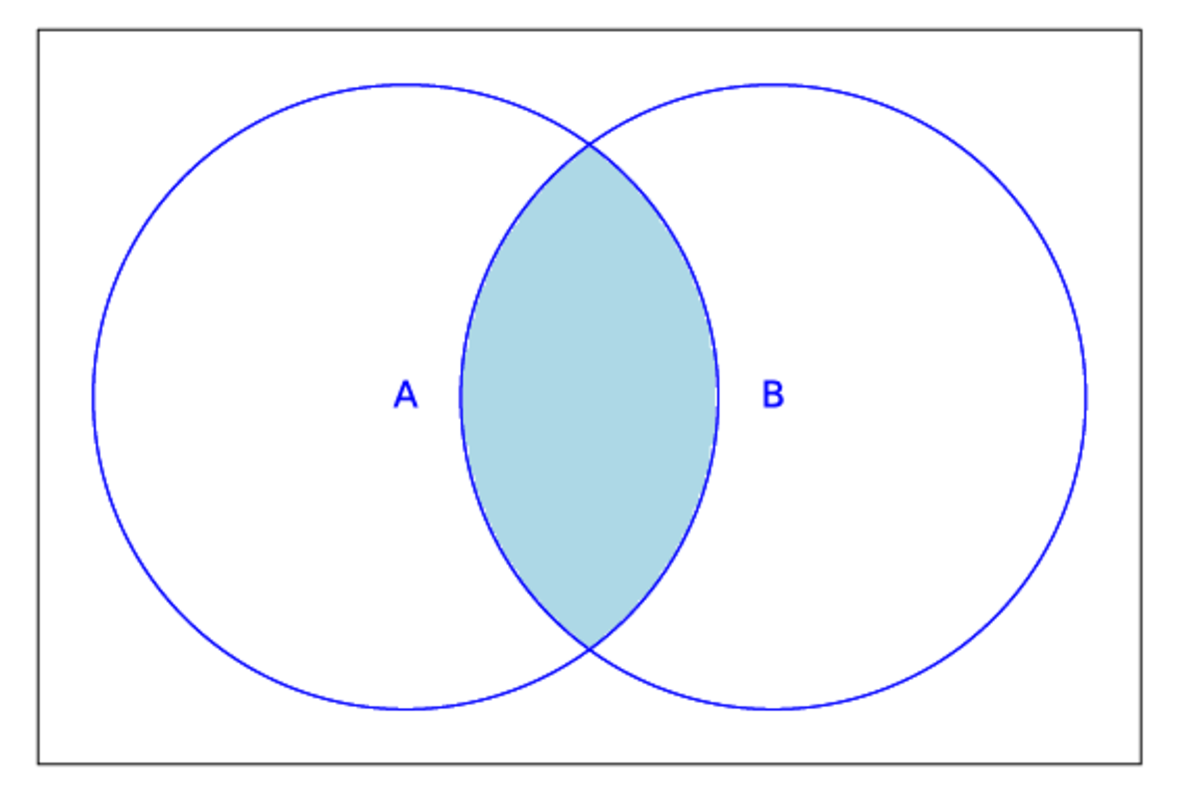
\includegraphics[width=0.80\textwidth]{images/sageplot-venn-intersection.pdf}}%
{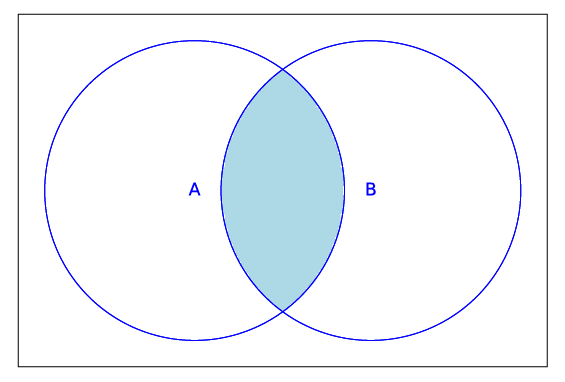
\includegraphics[width=0.80\textwidth]{images/sageplot-venn-intersection.png}}
\caption{Venn Diagram\label{venn_diagram_intersection}}
\end{figure}

 %
\par
(b) The union \(A \cup  B\) is illustrated in the following figure.
            \leavevmode%
\begin{figure}
\centering
\IfFileExists{images/sageplot-venn-union.pdf}%
{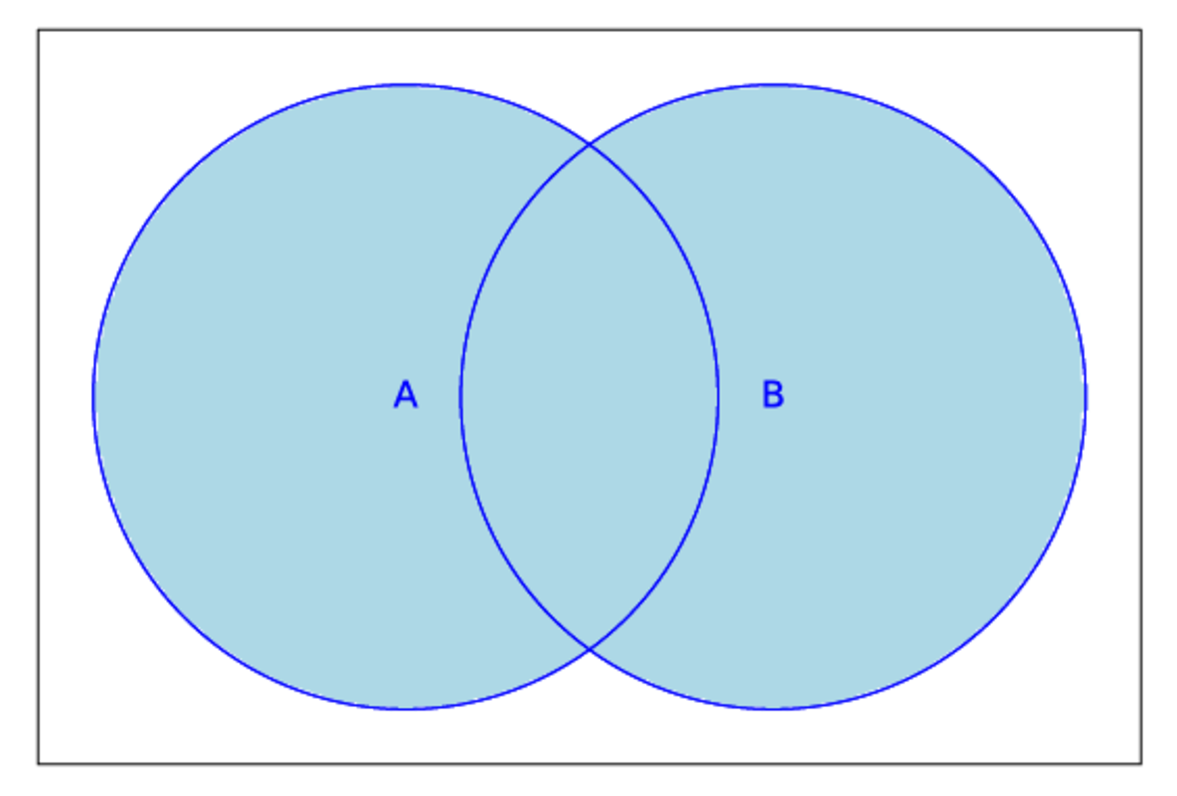
\includegraphics[width=0.80\textwidth]{images/sageplot-venn-union.pdf}}%
{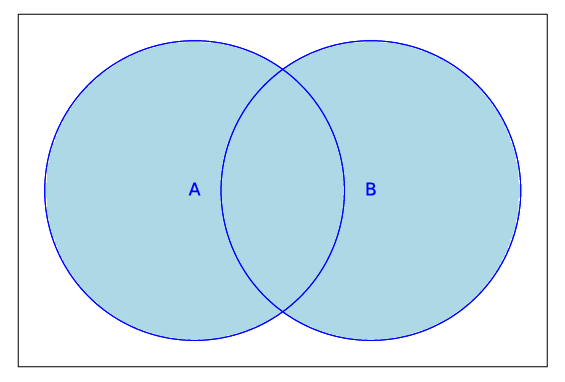
\includegraphics[width=0.80\textwidth]{images/sageplot-venn-union.png}}
\caption{Venn Diagram for the union \(A \cup  B\) \label{venn_diagram_union}}
\end{figure}
 
In a Venn diagram, the region representing \(A \cap  B\) does not appear empty; however, in some instances it will represent the empty set. The same is true for any other region in a Venn diagram. 
%
\end{example}
\begin{definition}[Complement of a set]\label{set_complement.}
Let \( A\) and \( B\) be sets. The complement of \( A\) relative to \( B\) (notation
\(B - A\)) is the set of elements that are in \( B\) and not in \( A\). That is, \(B-A=\{x: x\in B \textrm{ and } x\notin A\}\). If \(
U\) is the universal set, then \(U-A\) is denoted by \(A^c\) and is called simply the complement of \( A\). \(A^c=\{x\in U : x\notin A\}\). 
\end{definition}
\label{notation-5}
\begin{example}[Some Complements]\label{complements}
\leavevmode%
\begin{enumerate}
\item\hypertarget{li-55}{} Let \(U = \{1,2, 3, \text{...} , 10\}\) and \(A = \{2,4,6,8, 10\}\). Then \(U-A = \{1, 3, 5, 7, 9\}\) and \(A - U= \emptyset\)
\item\hypertarget{li-56}{} If \(U = \mathbb{R}\), then the complement of the rational numbers is the irrational numbers. 
\item\hypertarget{li-57}{} \(U^c= \emptyset\) and \(\emptyset ^c= U\). 
\item\hypertarget{li-58}{} The Venn diagram of \(B - A\) is represented in the following figure. 
            \leavevmode%
\begin{figure}
\centering
\IfFileExists{images/sageplot-venn-complement1.pdf}%
{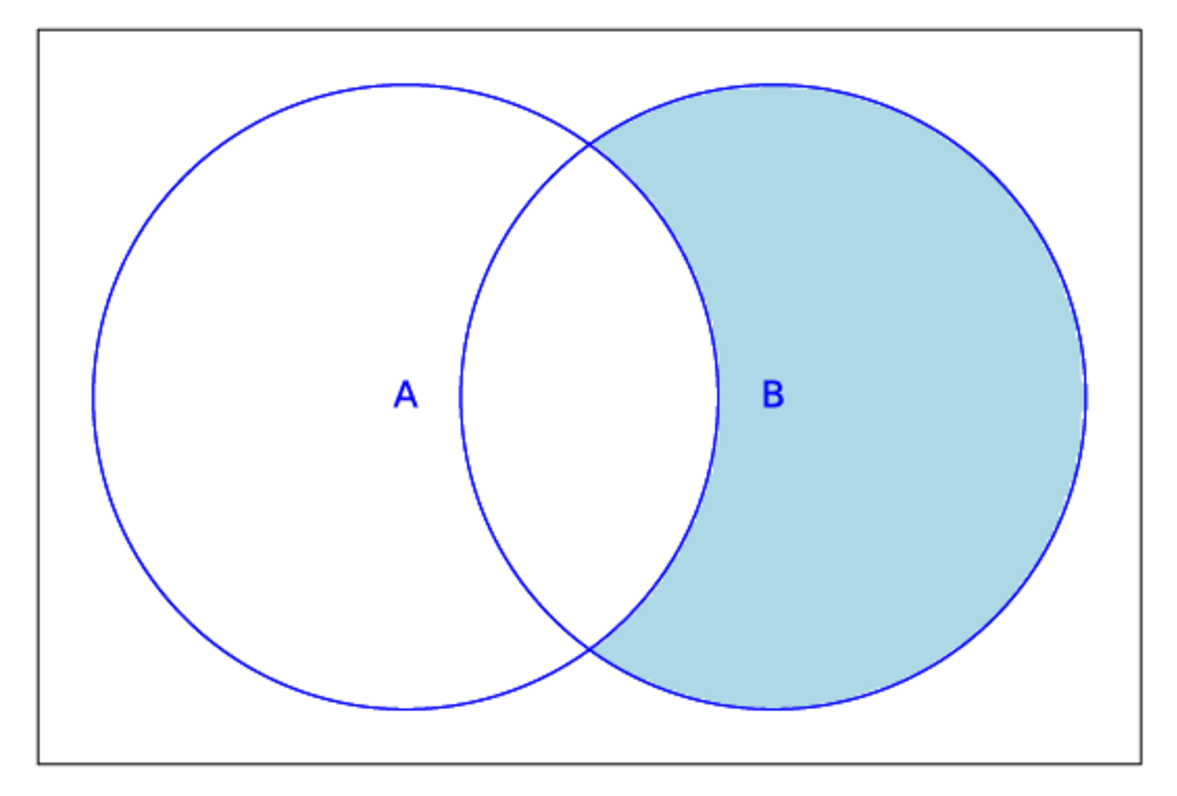
\includegraphics[width=0.80\textwidth]{images/sageplot-venn-complement1.pdf}}%
{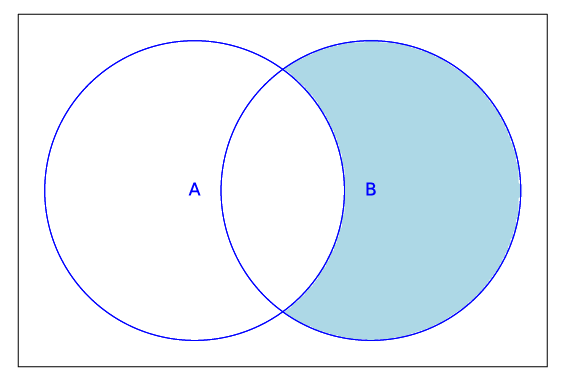
\includegraphics[width=0.80\textwidth]{images/sageplot-venn-complement1.png}}
\caption{Venn Diagram for \(B - A\)\label{venn_diagram_complement1}}
\end{figure}
 
\item\hypertarget{li-59}{} The Venn diagram of \(A^c\) is represented in the figure below. 
            \leavevmode%
\begin{figure}
\centering
\IfFileExists{images/sageplot-venn-complement2.pdf}%
{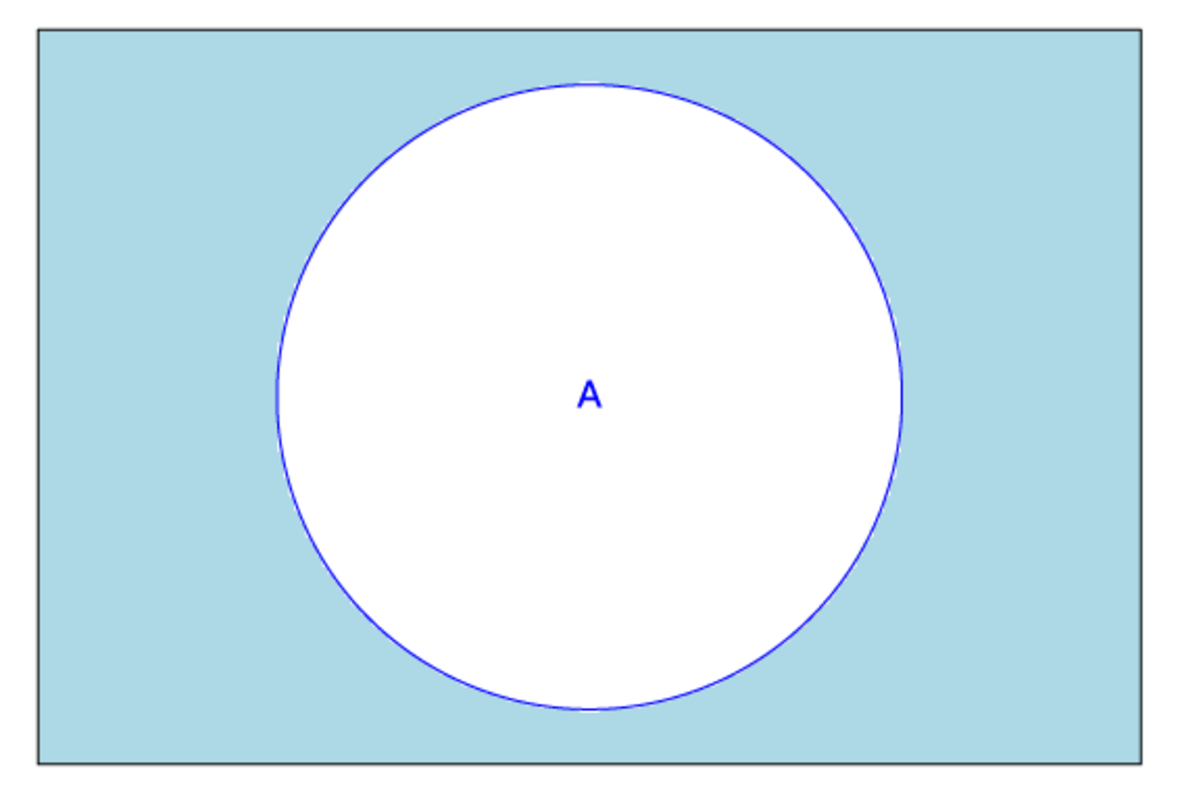
\includegraphics[width=0.80\textwidth]{images/sageplot-venn-complement2.pdf}}%
{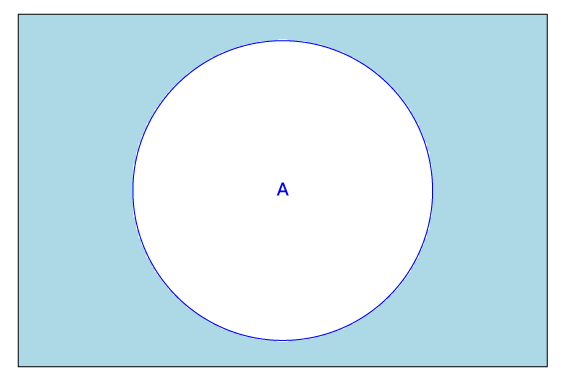
\includegraphics[width=0.80\textwidth]{images/sageplot-venn-complement2.png}}
\caption{Venn Diagram for \(A^{c}\)\label{venn_diagram_complement2}}
\end{figure}
 
\item\hypertarget{li-60}{} If \(B\subseteq A\), then the Venn diagram of \(A- B\) is as shown in the following figure.   
            \leavevmode%
\begin{figure}
\centering
\IfFileExists{images/sageplot-venn-complement3.pdf}%
{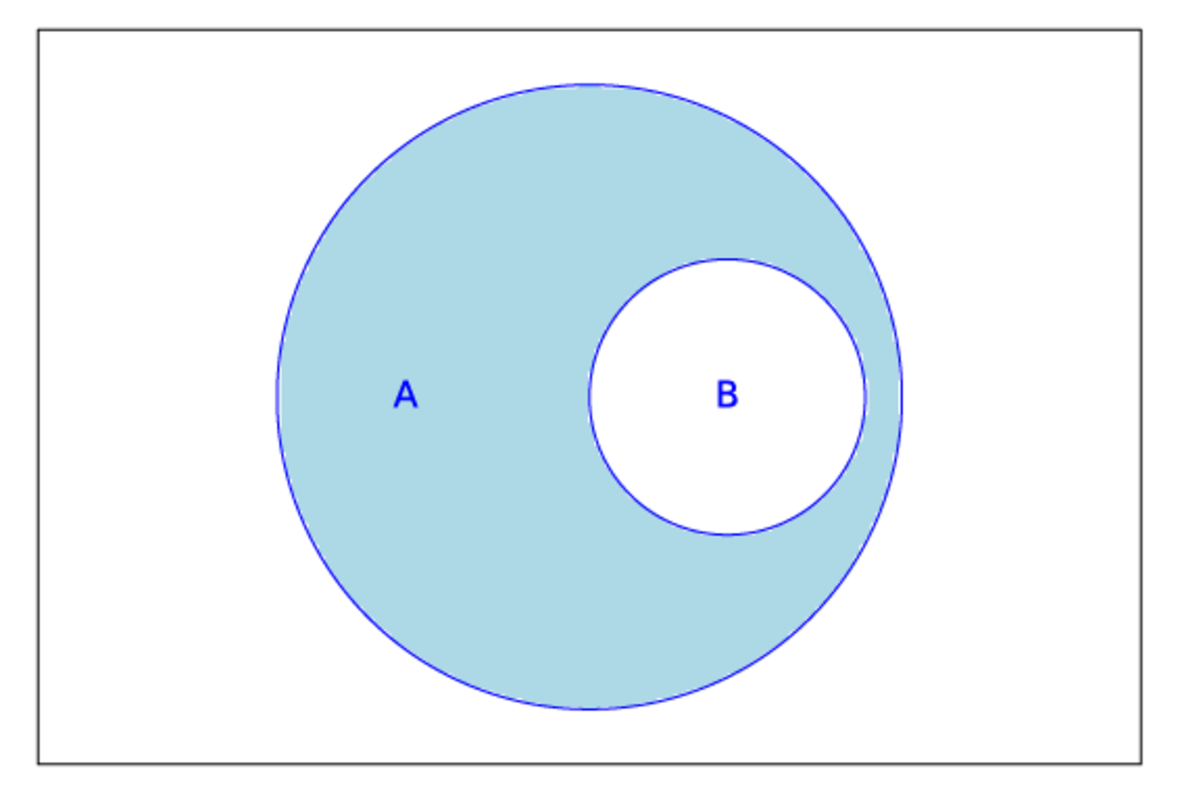
\includegraphics[width=0.80\textwidth]{images/sageplot-venn-complement3.pdf}}%
{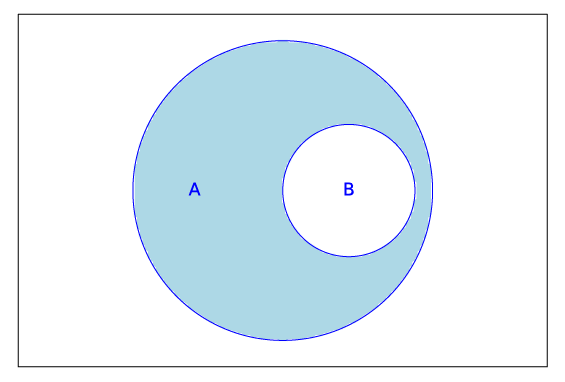
\includegraphics[width=0.80\textwidth]{images/sageplot-venn-complement3.png}}
\caption{Venn Diagram for \(A^{c}\)\label{venn_diagram_complement3}}
\end{figure}
 
\item\hypertarget{li-61}{} In the universe of integers, the set of even integers, \(\{\ldots  , - 4,-2, 0, 2, 4,\ldots \}\), has the set of odd integers as its complement.
\end{enumerate}
\end{example}
\begin{definition}[ Symmetric Difference.]\label{symmetric-difference.}
Let A and B be sets. The symmetric difference of A and B (denoted by \(A\oplus B\)) is the set of all elements
that are in AandB but not in both. That is, \(A \oplus  B = (A \cup  B) - (A \cap  B)\). 
\end{definition}
\label{notation-6}
\begin{example}[Some Symmetric Differences]\label{some_symmetric_differences}
\leavevmode%
\begin{enumerate}
\item\hypertarget{li-62}{}Let \(A = \{1, 3, 8\}\) and \(B = \{2, 4, 8\}\). Then \(A \oplus  B = \{1, 2, 3, 4\}\). 
\item\hypertarget{li-63}{}\(A \oplus  0 = A\) and \(A \oplus  A = \emptyset\) for any set \(A\). 
\item\hypertarget{li-64}{}\(\mathbb{R} \oplus  \mathbb{Q}\) is the set of irrational numbers. 
\item\hypertarget{li-65}{}The Venn diagram of \(A \oplus  B\) is represented in the following figure.
            \leavevmode%
\begin{figure}
\centering
\IfFileExists{images/sageplot-venn-symmetric.pdf}%
{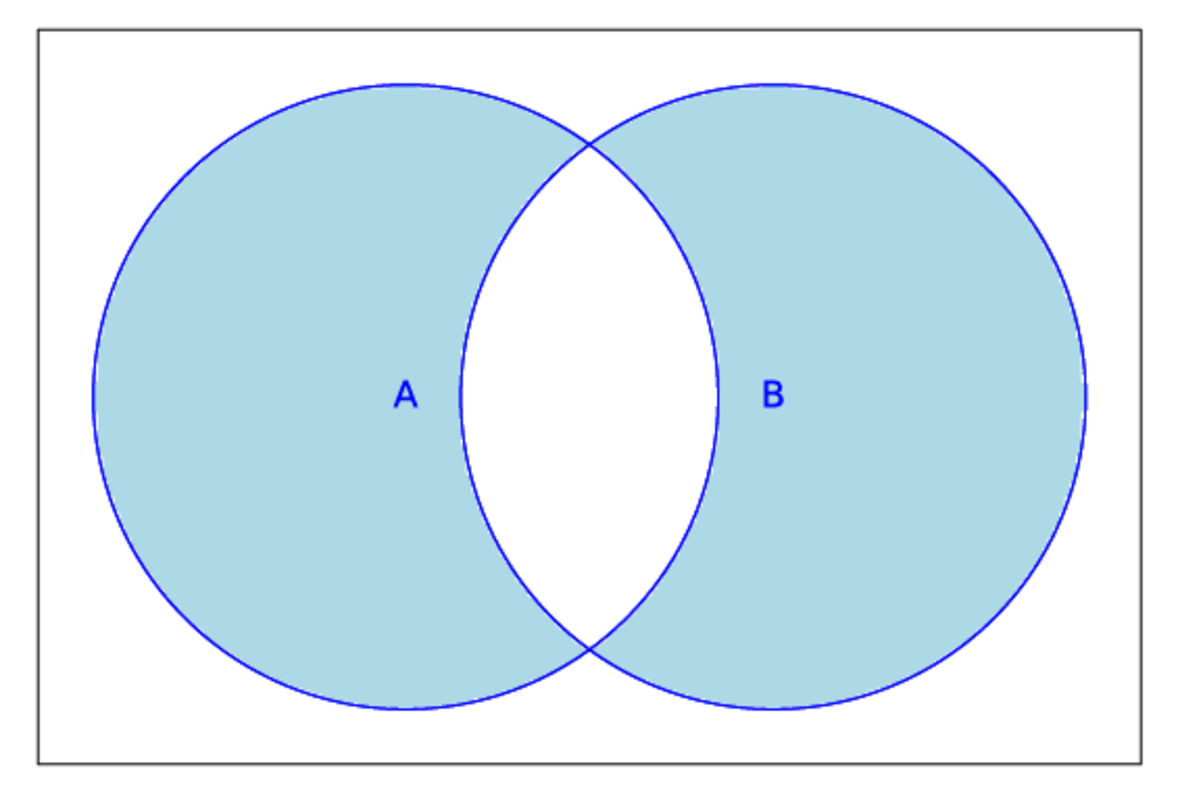
\includegraphics[width=0.80\textwidth]{images/sageplot-venn-symmetric.pdf}}%
{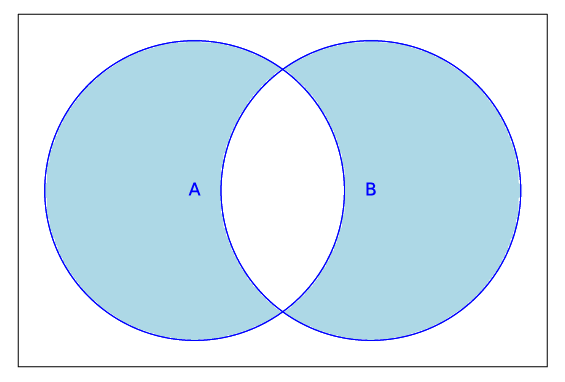
\includegraphics[width=0.80\textwidth]{images/sageplot-venn-symmetric.png}}
\caption{Venn Diagram for the symmetric difference \(A \oplus  B\)\label{venn_diagram_symmetric}}
\end{figure}
 
 %
  
\end{enumerate}
\end{example}
\typeout{************************************************}
\typeout{Subsubsection 1.2.2.1  \( Sage\) Note: Sets}
\typeout{************************************************}
\subsubsection[ \( Sage\) Note: Sets]{ \( Sage\) Note: Sets}\label{subsubsection-1}
To work with sets in Sage, a set is an expression of the form  Set(\emph{list}).  By wrapping a list with set, the order of elements appearing in the list and their duplication are ignored.  For example, L1 and L2 are two different list, but notice how as sets they are considered equal:%
\begin{lstlisting}[style=sageinput]
L1=[3,6,9,0,3]
L2=[9,6,3,0,9]
[L1==L2, Set(L1)==Set(L2) ]
\end{lstlisting}
\par
The standard set operations are all methods and/or functions that can act on Sage sets. \emph{You need to evalute the following cell to use the subsequent cell.}%
\begin{lstlisting}[style=sageinput]
A=Set(srange(5,50,5))
B=Set(srange(6,50,6))
[A,B]
\end{lstlisting}
\par

We can test membership, asking whether 10 is in each of the sets:
%
\begin{lstlisting}[style=sageinput]
[10 in A, 10 in B]
\end{lstlisting}
\par

The ampersand is used for the intersection of sets.  Change it to the vertical bar, |,  for intersection. 
%
\begin{lstlisting}[style=sageinput]
A & B
\end{lstlisting}
\par
Symmetric difference is defined as a &method& in Sage. To compute the symmetric difference of A  with  B, we evaluate the expression \(\texttt{ A.symmetric_difference(B) }\).%
\typeout{************************************************}
\typeout{Exercises 1.2.3 EXERCISES FOR SECTION 1.2 }
\typeout{************************************************}
\subsection[EXERCISES FOR SECTION 1.2 ]{EXERCISES FOR SECTION 1.2 }\label{exercises-1.2}
\hypertarget{exercisegroup-3}{}\typeout{************************************************}
\typeout{Introduction  }
\typeout{************************************************}
A Exercises%
\begin{exercisegroup}
\item[1.]\hypertarget{exercise-7}{} Let \(A = \{0, 2, 3\}\), \(B = \{2, 3\}\), \(C = \{1, 5, 9\}\), and let the universal set be \(U = \{0, 1, 2, . . . , 9\}\). Determine: 
\leavevmode%
\begin{multicols}{2}
\begin{enumerate}[label=(\alph*)]
\item\hypertarget{li-66}{}  \(A \cap  B\)  \item\hypertarget{li-67}{}  \(A \cup  B\)\item\hypertarget{li-68}{}  \(B \cup  A\)   \item\hypertarget{li-69}{}  \(A \cup  C\) \item\hypertarget{li-70}{}  \(A - B\)\item\hypertarget{li-71}{}  \(B - A\)\item\hypertarget{li-72}{}   \(A^c\) \item\hypertarget{li-73}{}   \(C^c\)\item\hypertarget{li-74}{}  \(A\cap C\)\item\hypertarget{li-75}{}   \(A\oplus B\) \end{enumerate}
\end{multicols}
\par\smallskip
\item[2.]\hypertarget{exercise-8}{}  Let \( A\), \( B\), and \( C\) be as in Exercise 1, let \(D = \{3, 2\}\), and let \(E = \{2, 3, 2\}\). Determine which of the
following are true. Give reasons for your decisions. 
\leavevmode%
\begin{multicols}{2}
\begin{enumerate}[label=(\alph*)]
\item\hypertarget{li-76}{}  \(A = B\) \item\hypertarget{li-77}{}  \(B = C\) \item\hypertarget{li-78}{}  \(B = D\) \item\hypertarget{li-79}{}  \(E=D\)\item\hypertarget{li-80}{}  \(A\cap B = B\cap A\)\item\hypertarget{li-81}{}  \(A \cup  B = B \cup  A\) \item\hypertarget{li-82}{}  \(A-B = B-A\) \item\hypertarget{li-83}{}  \(A \oplus  B = B \oplus  A\) \end{enumerate}
\end{multicols}
\par\smallskip
\item[3.]\hypertarget{exercise-9}{}  Let \(U= \{1, 2, 3, . . . , 9\}\). 
Give examples of sets \( A\), \( B\), and \( C\) for which:
\leavevmode%
\begin{multicols}{2}
\begin{enumerate}[label=(\alph*)]
\item\hypertarget{li-84}{}  \(A\cap (B\cap C)=(A\cap B)\cap C\) \item\hypertarget{li-85}{}  \(A\cap (B\cup C)=(A\cap B)\cup (A\cap C)\)\item\hypertarget{li-86}{}  \((A \cup  B)^c= A^c\cap B^c\) \item\hypertarget{li-87}{}  \(A \cup  A^c = U\)\item\hypertarget{li-88}{}  \(A \subseteq A\cup B\)\item\hypertarget{li-89}{}  \(A\cap B \subseteq A\) \end{enumerate}
\end{multicols}
\par\smallskip
\item[4.]\hypertarget{exercise-10}{}  Let \(U= \{1, 2, 3, . . . , 9\}\). Give examples to illustrate the following facts: 
\leavevmode%
\begin{multicols}{1}
\begin{enumerate}[label=(\alph*)]
\item\hypertarget{li-90}{}  If \(A \subseteq  B\) and \(B \subseteq C\), then \(A\subseteq C\).\item\hypertarget{li-91}{}  \(A - B \neq  B - A\) \item\hypertarget{li-92}{}  If \(U = A\cup  B\) and \(\text{A $\cap $ B = $\emptyset $}\), it always follows that \(A = U - B\). \item\hypertarget{li-93}{}  \(A \times  (B\cap C) = (A \times  B)\cap  (A \times C)\)   \end{enumerate}
\end{multicols}
\par\smallskip
\end{exercisegroup}
\par\smallskip\noindent
\hypertarget{exercisegroup-4}{}\typeout{************************************************}
\typeout{Introduction  }
\typeout{************************************************}
B Exercises%
\begin{exercisegroup}
\item[5.]\hypertarget{exercise-11}{}  What can you say about \(A\) if \(U = \{1, 2, 3, 4, 5\}\), \(B = \{2, 3\}\), and (separately) 
\leavevmode%
\begin{multicols}{1}
\begin{enumerate}[label=(\alph*)]
\item\hypertarget{li-94}{}  \(A \cup B = \{1, 2, 3,4\}\) \item\hypertarget{li-95}{}  \(A \cap  B = \{2\}\) \item\hypertarget{li-96}{}  \(A \oplus  B = \{3, 4, 5\}\)\end{enumerate}
\end{multicols}
\par\smallskip
\item[6.]\hypertarget{exercise-12}{} Suppose that \( U\) is an infinite universal set, and \( A\) and \( B\) are infinite subsets of \( U\). Answer the following questions with a brief explanation. 
\leavevmode%
\begin{multicols}{1}
\begin{enumerate}[label=(\alph*)]
\item\hypertarget{li-97}{}  Must \(A^c\) be finite? \item\hypertarget{li-98}{}  Must \(A\cup B\) infinite? \item\hypertarget{li-99}{}  Must \(A\cap B\) be infinite? \end{enumerate}
\end{multicols}
\par\smallskip
\item[7.]\hypertarget{exercise-13}{}  Given that \( U\) = all students at a university, \( D\) = day students, \( M\) = mathematics majors, and \( G\) = graduate
students. Draw Venn diagrams illustrating this situation and shade in the following sets: 
\leavevmode%
\begin{multicols}{1}
\begin{enumerate}[label=(\alph*)]
\item\hypertarget{li-100}{}  evening students \item\hypertarget{li-101}{}  undergraduate mathematics majors \item\hypertarget{li-102}{}  non-math graduate students \item\hypertarget{li-103}{}  non-math undergraduate students\end{enumerate}
\end{multicols}
\par\smallskip
\item[8.]\hypertarget{exercise-14}{} Let the sets \( D\), \( M\), \( G\), and \( U\) be as in exercise 7.  Let \(\lvert U \rvert  = 16,000\), \(\lvert D \rvert = 9,000\), \(|M |=
300\), and \(\lvert G \rvert = 1,000\). Also assume that the number of day students who are mathematics majors is 250, fifty of whom are graduate students, that there are 95 graduate mathematics majors, and that the total number of day graduate students is 700. Determine the number of students who are: 
\leavevmode%
\begin{multicols}{1}
\begin{enumerate}[label=(\alph*)]
\item\hypertarget{li-104}{}  evening students \item\hypertarget{li-105}{}  nonmathematics majors \item\hypertarget{li-106}{}  undergraduates (day or evening) \item\hypertarget{li-107}{}  day graduate nonmathematics majors \item\hypertarget{li-108}{}  evening graduate students \item\hypertarget{li-109}{}  evening graduate mathematics majors \item\hypertarget{li-110}{}  evening undergraduate nonmathematics majors \end{enumerate}
\end{multicols}
\par\smallskip
\end{exercisegroup}
\par\smallskip\noindent
\typeout{************************************************}
\typeout{Section 1.3 Cartesian Products and Power Sets}
\typeout{************************************************}
\section[Cartesian Products and Power Sets]{Cartesian Products and Power Sets}\label{Cartesian_Products_and_Power_Sets}
\begin{definition}[ Cartesian Product.]\label{cartesian-product.}
 Let \(A\) and \(B\) be sets. The Cartesian product of \(A\) and \(B\), denoted by \(A\times B\), is defined as follows: \(A\times B = \{(a, b) \mid a \in  A \quad\textrm{ and }\quad b \in  B\}\), that is, \(A\times B\) is the set of all possible ordered pairs whose first component comes from \(A\) and whose second component comes from \(B\).
 \end{definition}
\begin{example}[Some Cartesian Products]\label{example-8}
 Notation in mathematics is often developed for good reason. In this case, a few examples will make clear why the symbol $\times $ is used for Cartesian products.%
\leavevmode%
\begin{itemize}[label=\textbullet]
\item{}  Let \(A = \{1, 2, 3\}\) and \(B = \{4, 5\}\). Then \(A \times  B = \{(1, 4), (1, 5), (2, 4), (2, 5), (3, 4), (3, 5)\}\). Note that \(|A \times B| = 6 = \lvert A \rvert  \times  \lvert B \rvert \). \item{}  \(A \times  A = \{(1, 1), (1, 2), (1, 3), (2, 1), (2, 2), (2, 3), (3, 1), (3, 2), (3, 3)\}\). Note that \(|A \times  A| = 9 = {\lvert A \rvert}^2\).\end{itemize}
\end{example}
These two examples illustrate the general rule: If A and B are finite sets, then \(| A \times B | = \lvert A \rvert  \times  \lvert B \rvert \).%
\par
We can define the Cartesian product of three (or more) sets similarly. For example, \(A \times  B \times  C = \{(a, b, c):a \in  A, b \in  B, c \in C\}\). %
\par
It is common to use exponents if the sets in a Cartesian product are the same: 
\[A^2= A \times  A\]
\[A^3=A \times A \times A\]
and in general, 
\[A^n =A \times A \times \ldots \times A\].%
\typeout{************************************************}
\typeout{Subsection 1.3.1 Power Sets}
\typeout{************************************************}
\subsection[Power Sets]{Power Sets}\label{subsection-5}
\begin{definition}[ Power Set. ]\label{power-set}
If \( A\) is any set, the power set of \(A\) is the set of all subsets of \(A\), denoted \(\mathcal{P}(A)\).\end{definition}
\label{notation-7}
\par
The two extreme cases, the empty set and all of \(A\), are both included in \(\mathcal{P}(A)\).%
\begin{example}[ Some Power Sets ]\label{Some_Power_Sets}
\leavevmode%
\begin{itemize}[label=\textbullet]
\item{}\(\mathcal{P}(\emptyset )=\{\emptyset \}\) \item{} \(\mathcal{P}(\{1\}) = \{\emptyset , \{1\}\}\) \item{} \(\mathcal{P}(\{1,2\}) = \{\emptyset , \{1\}, \{2\}, \{1, 2\}\}\). \end{itemize}
We will leave it to you to guess at a general formula for the number of elements in the power set of a finite set. In Chapter 2, we will discuss counting rules that will help us derive this formula.%
\end{example}
\typeout{************************************************}
\typeout{Subsubsection 1.3.1  \( Sage\) Note: Cartesion Products and Power Sets}
\typeout{************************************************}
\subsection[ \( Sage\) Note: Cartesion Products and Power Sets]{ \( Sage\) Note: Cartesion Products and Power Sets}\label{subsubsection-2}
Here is a simple example of a cartesion product of two sets:%
\begin{lstlisting}[style=sageinput]
A=Set([0,1,2])
B=Set(['a','b'])
P=cartesian_product([A,B]);P
\end{lstlisting}
\par
Here is the cardinality of the cartesian product.%
\begin{lstlisting}[style=sageinput]
P.cardinality()
\end{lstlisting}
\par

The power set of a set is an iterable, as you can see from the output of this next cell
%
\begin{lstlisting}[style=sageinput]
U=Set([0,1,2,3])
subsets(U)
\end{lstlisting}
\par

You can iterate over a powerset - here is a trivial example.  
%
\begin{lstlisting}[style=sageinput]
for a in subsets(U):
    print(str(a)+ " has " +str(len(a))+" elements.")
\end{lstlisting}
\typeout{************************************************}
\typeout{Exercises 1.3.3 EXERCISES FOR SECTION 1.3 }
\typeout{************************************************}
\subsection[EXERCISES FOR SECTION 1.3 ]{EXERCISES FOR SECTION 1.3 }\label{exercises-1.3}
\hypertarget{exercisegroup-5}{}\typeout{************************************************}
\typeout{Introduction  }
\typeout{************************************************}
A Exercises%
\begin{exercisegroup}
\item[1.]\hypertarget{exercise-15}{}  Let \(A = \{0, 2, 3\}\), \(B = \{2, 3\}\), \(C = \{1, 4\}\), and let the universal set be \(U = \{0, 1, 2, 3, 4\}\). List the elements of 
\leavevmode%
\begin{itemize}[label=\textbullet]
\item{}  \(A \times B\) \item{}  \(B \times  A\) \item{}  \(A \times B\times C\) \item{}  \(U \times \emptyset\)\item{}  \(A \times  A^c\)\item{}  \(B^2\) \item{}  \(B^3\)\item{}  \(B\times \mathcal{P}(B)\)\end{itemize}
\par\smallskip
\item[2.]\hypertarget{exercise-16}{} 
Suppose that you are about to flip a coin and then roll a die. Let \(A = \{HEADS, TAILS\}\) and  \(B = {$1, 2, 3, 4, 5, 6}\). 
\leavevmode%
\begin{itemize}[label=\textbullet]
\item{}  What is \(|A \times  B|\)? \item{}  How could you interpret the set \(A \times  B\) ?   \end{itemize}
\par\smallskip
\item[3.]\hypertarget{exercise-17}{} 
List all two-element sets in \(\mathcal{P}(\{a,b,c\})\)\par\smallskip
\item[4.]\hypertarget{exercise-18}{} 
List all three-element sets in \(\mathcal{P}(\{a, b, c,d\})\). 
\par\smallskip
\item[5.]\hypertarget{exercise-19}{} 
How many singleton (one-element) sets are there in \(\mathcal{P}(A)\) if \(\lvert A \rvert =n\) ? 
\par\smallskip
\item[6.]\hypertarget{exercise-20}{} 
A person has four coins in his pocket: a penny, a nickel, a dime, and a quarter. How many different sums of money can he take out if he removes
3 coins at a time? 
\par\smallskip
\item[7.]\hypertarget{exercise-21}{} 
Let \(A = \{+,-\}\) and \(B = \{00, 01, 10, 11\}\).
\leavevmode%
\begin{itemize}[label=\textbullet]
\item{}  List the elements of \(A \times  B\) \item{}  How many elements do \(A ^4\) and \((A \times B)^3\) have? \end{itemize}
\par\smallskip
\end{exercisegroup}
\par\smallskip\noindent
\hypertarget{exercisegroup-6}{}\typeout{************************************************}
\typeout{Introduction  }
\typeout{************************************************}
B Exercises%
\begin{exercisegroup}
\item[8.]\hypertarget{exercise-22}{} 
Let \(A = \{\bullet,\square ,\otimes \}\) and \(B = \{\square ,\ominus ,\bullet\}\). 
\leavevmode%
\begin{itemize}[label=\textbullet]
\item{} List the elements of \(A \times  B\) and \(B \times  A\). The parentheses and comma in an ordered pair are not necessary in cases such as this where the elements of each set are individual symbol. \item{}  Identify the intersection of \(A \times  B\) and \(B \times  A\). for the case above, and then guess at a general rule for the intersection of \(A \times  B\) and \(B \times  A\). where \( A\) and \( B\) are any two sets. \end{itemize}
\par\smallskip
\item[9.]\hypertarget{exercise-23}{} 
Let \(A\) and \(B\) be nonempty sets. When are \(A \times  B\) and \(B \times  A\). equal? 
\par\smallskip
\end{exercisegroup}
\par\smallskip\noindent
\typeout{************************************************}
\typeout{Section 1.4 Binary Representation of Positive Integers }
\typeout{************************************************}
\section[Binary Representation of Positive Integers ]{Binary Representation of Positive Integers }\label{Binary_Representation_of_Positive_Integers }
Recall that the set of positive integers, \(\mathbb{P}\), is \(\{1, 2, 3, . . . \}\). Positive integers are naturally used to count things. There are many ways to count and many ways to record, or represent, the results of counting. For example, if we wanted to count five hundred twenty-three apples, we might group the apples by tens. There would be fifty-two groups of ten with three single apples left over. The fifty-two groups of ten could be put into five groups of ten tens (hundreds), with two tens left over. The five hundreds, two tens, and three units is recorded as 523. This system of counting is called the base ten positional system, or decimal system. It is quite natural for us to do grouping by tens, hundreds, thousands, \(\dots\) since it is the method that all of us use in everyday life. %
\par
 The term positional refers to the fact that each digit in the decimal representation of a number has a significance based on its position. Of course this means that rearranging digits will change the number being described. You may have learned of numeraton systems in which the position of symbols does not have any significance (e.g., the ancient Egyptian system). Most of these systems are merely curiosities to us now.%
\par
The binary number system differs from the decimal number system in that units are grouped by twos, fours, eights, etc. That is, the group sizes are powers of two instead of powers of ten. For example, twenty-three can be grouped into eleven groups of two with one left over. The eleven twos can be grouped into five groups of four with one group of two left over. Continuing along the same lines, we find that twenty-three can be described as one sixteen, zero eights, one four, one two, and one one, which is abbreviated \(10111_{\textrm{two}}\), or simply \(10111\) if the
context is clear. %
\par
The process that we used to determine the binary representation of \(23\) can be described in general terms to determine the binary representation of any positive integer n. A general description of a process such as this one is called an algorithm. Since this is the first algorithm in the book, we will first write it out using less formal language than usual, and then introduce some ``algorithmic notation.''%
\par
\leavevmode%
\begin{enumerate}
\item\hypertarget{li-130}{} Start with an empty list of bits. \item\hypertarget{li-131}{} Step Two: Assign the variable \(k\) the value \(n\). \item\hypertarget{li-132}{} Step Three: While \(k\)'s value is positive, continue performing the following three steps until \(k\) becomes zero and then stop. 
	\begin{enumerate}
\item\hypertarget{li-133}{}divide \(k\) by 2, obtaining a quotient \(q\) (often denoted \(k \textrm{ div } 2\)) and a remainder \(r\) (denoted \((k \bmod 2)\)). \item\hypertarget{li-134}{}attach \(r\) to the left-hand side of the list of bits. \item\hypertarget{li-135}{} assign the variable \(k\) the value \(q\).\end{enumerate}
\end{enumerate}
%
\begin{example}[An example of conversion to binary]\label{An_example_of_conversion_to_binary}
 To determine the binary representation of 41 we take the following steps:
\leavevmode%
\begin{itemize}[label=\textbullet]
\item{}\(41 = 2 \times  20+ 1 \quad List = 1 \) \item{}\(20 = 2 \times  10+0 \quad List = 01 \)\item{} \(10 = 2\times 5 + 0 \quad List = 001 \)\item{}\(5 =\text2\times  2+ 1 \quad List =1001\) \item{}\(2 =2\times  1+ 0 \quad List = 01001 \)\item{}\(1 =\text2 \times 0\text+1  \quad List = 101001\) \end{itemize}
   
Therefore, \(41=101001_{\textrm{two}}\)%
\end{example}
\par
The notation that we will use to describe this algorithm and all others is called pseudocode, an informal variation of the instructions that are commonly used in many computer languages. Read the following description carefully, comparing it with the informal description above. Appendix B, which contains a general discussion of the components of the algorithms in this book, should clear up any lingering questions. Anything after // are comments.%
\begin{algorithm}[Binary Conversion Algorithm]\label{binary_conversion_algorithm}
 An algorithm for determining the binary representation of a positive integer.%
\par
Input: a positive integer n.%
\par
Output: the binary representation of n in the form of a list of bits, with units bit last, twos bit next to last, etc.%
\leavevmode%
\begin{enumerate}
\item\hypertarget{li-142}{}k := n \(\qquad  \)     //initialize k\item\hypertarget{li-143}{}L := { } \(\qquad  \)   //initialize L to an empty list\item\hypertarget{li-144}{} While k > 0 do 
   \begin{enumerate}
\item\hypertarget{li-145}{} q := k div 2		\(\qquad  \)	//divide k by 2\item\hypertarget{li-146}{} r:= k mod 2 \item\hypertarget{li-147}{}L: = prepend r to L \(\qquad  \) //Add r to the front of L \item\hypertarget{li-148}{} k:= q   			\(\qquad  \)	//reassign k\end{enumerate}
\end{enumerate}
\end{algorithm}
\par
Now that you've read this section, you should get this joke.%
\leavevmode%
\begin{figure}
\centering
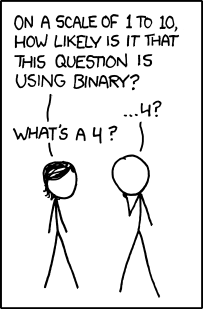
\includegraphics[width=300pt,]{images/1_to_10.png}\caption{With permission from Randall Munroe
                \label{onetoten}}
\end{figure}
\typeout{************************************************}
\typeout{Exercises 1.4.1 EXERCISES FOR SECTION 1.4 }
\typeout{************************************************}
\subsection[EXERCISES FOR SECTION 1.4 ]{EXERCISES FOR SECTION 1.4 }\label{exercises-1.4}
\hypertarget{exercisegroup-7}{}\typeout{************************************************}
\typeout{Introduction  }
\typeout{************************************************}
A Exercises%
\begin{exercisegroup}
\item[1.]\hypertarget{exercise-24}{} 
Find the binary representation of each of the following positive integers: 
\leavevmode%
\begin{enumerate}[label=(\alph*)]
\item\hypertarget{li-149}{} 31\item\hypertarget{li-150}{} 32\item\hypertarget{li-151}{}10\item\hypertarget{li-152}{}100 \end{enumerate}
\par\smallskip
\item[2.]\hypertarget{exercise-25}{} 
Find the binary representation of each of the following positive integers: 
\leavevmode%
\begin{enumerate}[label=(\alph*)]
\item\hypertarget{li-153}{} 64\item\hypertarget{li-154}{} 67\item\hypertarget{li-155}{}28\item\hypertarget{li-156}{}256 \end{enumerate}
\par\smallskip
\item[3.]\hypertarget{exercise-26}{} 
What positive integers have the following binary representations?
\leavevmode%
\begin{enumerate}[label=(\alph*)]
\item\hypertarget{li-157}{} 10010\item\hypertarget{li-158}{} 10011\item\hypertarget{li-159}{}101010\item\hypertarget{li-160}{}10011110000 \end{enumerate}
\par\smallskip
\item[4.]\hypertarget{exercise-27}{} 
What positive integers have the following binary representations?
\leavevmode%
\begin{enumerate}[label=(\alph*)]
\item\hypertarget{li-161}{} 100001\item\hypertarget{li-162}{} 1001001\item\hypertarget{li-163}{}1000000000\item\hypertarget{li-164}{}1001110000 \end{enumerate}
\par\smallskip
\item[5.]\hypertarget{exercise-28}{} 
The number of bits in the binary representations of integers increase by one as the numbers double.  Using this fact, determine how many bits the binary representations of the following decimal numbers have without actually doing the full conversion. 
\( \quad (a) 2011  \quad (b)  4000   \quad (c) 4500   \quad (d) 2^{50}\)\par\smallskip
\end{exercisegroup}
\par\smallskip\noindent
\hypertarget{exercisegroup-8}{}\typeout{************************************************}
\typeout{Introduction  }
\typeout{************************************************}
B Exercises%
\begin{exercisegroup}
\item[6.]\hypertarget{exercise-29}{} 
Let \(m\) be a positive integer with \( n\)-bit binary representation: \(a_{n-1}a_{n-2}\cdots  a_1a_0\) with \(a_{n-1}=1\) What are the smallest
and largest values that \(m\) could have? 
\par\smallskip
\item[7.]\hypertarget{exercise-30}{} 
If a positive integer is a multiple of 100, we can identify this fact from its decimal representation, since it will end with two zeros. What can
you say about a positive integer if its binary representation ends with two zeros? 
\par\smallskip
\item[8.]\hypertarget{exercise-31}{} 
Can a multiple of ten be easily identified from its binary representation? 
\par\smallskip
\end{exercisegroup}
\par\smallskip\noindent
\typeout{************************************************}
\typeout{Section 1.5 Summation Notation and Generalizations }
\typeout{************************************************}
\section[Summation Notation and Generalizations ]{Summation Notation and Generalizations }\label{Summation_Notation_and_Generalizations }
Most operations such as addition of numbers are introduced as binary operations. That is, we are taught that two numbers may be added
together to give us a single number. Before long, we run into situations where more than two numbers are to be added. For example, if four numbers,
\(a_1\), \(a_2\), \(a_3\), and \(a_4\) are to be added, their sum may be written down in several ways, such as\(\) \(((a_1+a_2)+a_3)+a_4\)
or \(\left(a_1+a_2\right)+\left(a_3+a_4\right)\). In the first expression, the first two numbers are added, the result is added to the third number,
and that result is added to the fourth number. In the second expression the first two numbers and the last two numbers are added and the results
of these additions are added. Of course, we know that the final results will be the same. This is due to the fact that addition of numbers is an
associative operation. For such operations, there is no need to describe how more than two objects will be operated on. 
A sum of numbers such as \(a_1+a_2+a_3+a_4\)is called a series and is often written \(\sum _{k=1}^4 a_k\) in what is called \emph{ summation notation}. %
\par
We first recall some basic facts about series that you probably have seen before. A more formal treatment of sequences and series is covered in Chapter 8. The purpose here is to give the reader a working knowledge of summation notation and to carry this notation through to intersection
and union of sets and other mathematical operations. %
\par
A \emph{finite series} is an expression such as \(a_1+a_2+a_3 +\dots +a_n=\sum _{k=1}^{n} a_k\)%
\par
In the expression \(\sum _{k=1}^{n} a_k\):
\leavevmode%
\begin{itemize}[label=\textbullet]
\item{} The variable \(k\) is referred to as the \emph{ index}, or the index of summation.\item{} The expression \(a_k\) is the \emph{ general term} of the series. It defines the numbers that are being added together in the series.\item{} The value of \(k\) below the summation symbol is the \emph{ initial index} and the value above the summation symbol is the \emph{ terminal index}.\item{} It is understood that the series is a sum of the general terms where the index start with the initial index and increases by one up to and including the terminal index.\end{itemize}
%
\begin{example}[Some finite series]\label{some_finite_series}
(a)  \(\sum _{i=1}^4 a_i= a_1+ a_2+a_3+a_4\)%
\par
(b) \(\sum _{k=0}^5 b_k=b_0+b_1+b_2+b_3+b_4+b_5\)%
\par
(c) \(\sum _{i=-2}^2 c_i=c_{-2}+c_{-1}+c_0+c_1+c_2\)%
\end{example}
\begin{example}[More finite series ]\label{more_finite_series}
If the general terms in a series are more specific, the sum can often be simplified. For example, 
\leavevmode%
\begin{enumerate}
\item\hypertarget{li-169}{} \(\sum _{i=1}^4 i^2=1^2+2^2+3^2+4^2=30\) \item\hypertarget{li-170}{} \(\sum _{i=1}^5 (2i-1)=(2\ 1-1)+(2\ 2-1)+(2\ 3-1)+(2\ 4-1)+(2\ 5-1)\\
\\
\quad \quad =1+3+5+7+9\\
\\
\quad \quad =25\)\end{enumerate}

%
\end{example}
\par
Summation notation can be generalized to many mathematical operations, for example, 
\(A_1\cap A_2\cap A_3\cap A_4=\underset{i=1}{\overset{4}{\cap }}A_i\) %
\begin{definition}[ Generalized Set Operations.]\label{generalized-set-operations}
Let \(A_1, A_2, \ldots , A_n\) be sets. Then: 
\leavevmode%
\begin{enumerate}
\item\hypertarget{li-171}{}  \(A_1\cap A_2\cap \cdots \cap A_n=\underset{i=1}{\overset{n}{\cap }}A_i\)\item\hypertarget{li-172}{}   \(A_1\cup A_2\cup \cdots \cup A_n=\underset{i=1}{\overset{n}{\cup }}A_i\)\item\hypertarget{li-173}{}   \(A_1\times A_2\times \cdots \times A_n=\underset{i=1}{\overset{n}{\times }}A_i\)\item\hypertarget{li-174}{}   \(A_1\oplus A_2\oplus \cdots \oplus A_n=\underset{i=1}{\overset{n}{\oplus }}A_i\)\end{enumerate}
\end{definition}
\begin{example}[Some generalized operations]\label{some_generalized_operations}
If \(A_1 = \{0, 2, 3\}\), \(A_2 = \{1, 2, 3, 6\}\), and \(A_3 = \{-1, 0, 3, 9\}\), then 
 \[\underset{i=1}{\overset{4}{\cap }}A_i=A_1\cap A_2\cap A_3=\{3\}\]
and
\[\underset{i=1}{\overset{4}{\cup }}A_i=A_1\cup A_2\cup A_3=\{-1,0,1,2,3,6,9\}\]
With this notation it is quite easy to write lengthy expressions in a fairly compact form. For example, the statement 
    \[A\cap \left(B_1\cup B_2\cup \cdots \cup B_n\right)= \left(A\cap B_1\right)\cup \left(A\cap B_2\right)\cup \cdots \cup \left(A\cap
B_n\right)\]
becomes 
   \[A \cap \left(\underset{i=1}{\overset{n}{\cup }}B_i\right)= \underset{i=1}{\overset{n}{\cup }}\left(A\cap B_n\right)\]%
\end{example}
\typeout{************************************************}
\typeout{Exercises 1.5.1 EXERCISES FOR SECTION 1.5 }
\typeout{************************************************}
\subsection[EXERCISES FOR SECTION 1.5 ]{EXERCISES FOR SECTION 1.5 }\label{exercises-1.5}
\hypertarget{exercisegroup-9}{}\begin{exercisegroup}
\item[1.]\hypertarget{exercise-32}{} 
Calculate the following series:
\leavevmode%
\begin{enumerate}[label=(\alph*)]
\item\hypertarget{li-175}{}  \(\sum _{i=1}^3 (2 + 3i)\)\item\hypertarget{li-176}{}  \(\sum _{i=-2}^1 i^2\) \item\hypertarget{li-177}{}  \(\sum _{j=0}^n 2^j\text{   }\) for \(n= 1, 2, 3, 4\)\item\hypertarget{li-178}{}  \(\sum _{k=1}^n (2k-1)\) for \(n = 1, 2, 3, 4\) \end{enumerate}
\par\smallskip
\item[2.]\hypertarget{exercise-33}{} Calculate the following series: 
\leavevmode%
\begin{enumerate}[label=(\alph*)]
\item\hypertarget{li-179}{}  \(\sum _{k=1}^3 i^n\) for\(n = 1, 2, 3, 4\) \item\hypertarget{li-180}{}  \(\sum _{i=1}^5 20\) \item\hypertarget{li-181}{}   \(\sum _{j=0}^3 \left(n^j+1\right)\) for \(n = 1, 2, 3,4\) \item\hypertarget{li-182}{}   \(\sum _{k=-n}^n k\) for \(n = 1, 2, 3, 4\) \end{enumerate}
\par\smallskip
\item[3.]\hypertarget{exercise-34}{}\leavevmode%
\begin{enumerate}[label=(\alph*)]
\item\hypertarget{li-183}{}  Express the formula \(\sum _{i=1}^n \frac{1}{i(i+1)}= \frac{n}{n+1}\)  without using summation notation. \item\hypertarget{li-184}{}  Verify this formula for \(n=3\). \item\hypertarget{li-185}{}  Repeat parts (a) and (b) for \(\sum _{i=1}^n i^3=\frac{n^2(n+1)^2}{4}\)\end{enumerate}
\par\smallskip
\item[4.]\hypertarget{exercise-35}{}   Verify the following properties for \(n = 3\).   
\leavevmode%
\begin{enumerate}[label=(\alph*)]
\item\hypertarget{li-186}{}   \(\sum _{i=1}^n \left(a_i+ b_i\right) =\sum _{i=1}^n a_i +\sum _{i=1}^n  b_i\) \item\hypertarget{li-187}{}    \(c\left(\sum _{i=1}^n a_i\right) = \sum _{i=1}^n c a_i\)\end{enumerate}
\par\smallskip
\item[5.]\hypertarget{exercise-36}{} 
 Rewrite the following without summation sign for \(n = 3\). It is not necessary that you understand or expand the notation \(\left(
\begin{array}{c}
 n \\
 k \\
\end{array}
\right)\) at this point. 
  \((x + y)^n= \sum _{k=0}^n \left(
\begin{array}{c}
 n \\
 k \\
\end{array}
\right)x^{n-k}y^k\)\par\smallskip
\item[6.]\hypertarget{exercise-37}{}\leavevmode%
\begin{enumerate}[label=(\alph*)]
\item\hypertarget{li-188}{}  Draw the Venn diagram for \(\underset{i=1}{\overset{3}{\cap }}A_i\).\item\hypertarget{li-189}{} (b) Express in ``expanded format'': 
\(	A\cup (\underset{i=1}{\overset{n}{\cap }}B_i)= \underset{i=1}{\overset{n}{\cap }}(A \cup B_n)\).\end{enumerate}
\par\smallskip
\item[7.]\hypertarget{exercise-38}{} 
 For any positive integer \(k\), let \(A_k = \{x \in \mathbb{Q}:k-1 < x <= k\}\) and \(B_k = \{x \in \mathbb{Q}: -k < x < k\}\). What are
the following sets? 
\leavevmode%
\begin{enumerate}[label=(\alph*)]
\item\hypertarget{li-190}{}  \(\underset{i=1}{\overset{5}{\cup }}A_i\)\item\hypertarget{li-191}{}  \(\underset{i=1}{\overset{5}{\cup }}B_i\)\item\hypertarget{li-192}{}  \(\underset{i=1}{\overset{5}{\cap }}A_i\)\item\hypertarget{li-193}{}  \(\underset{i=1}{\overset{5}{\cap }}B_i\) \end{enumerate}
\par\smallskip
\item[8.]\hypertarget{exercise-39}{} 
 For any positive integer k, let \(A = \{x \in \mathbb{Q}:\text0 < x < 1/k\}\) and \(B _k = \{x \in \mathbb{Q}:\text{   }0 < x < k\}\). What
are the following sets? 
\leavevmode%
\begin{enumerate}[label=(\alph*)]
\item\hypertarget{li-194}{}  \(\underset{i=1}{\overset{\infty }{\cup }}A_i\)\item\hypertarget{li-195}{}  \(\underset{i=1}{\overset{\infty }{\cup }}B_i\)\item\hypertarget{li-196}{}  \(\underset{i=1}{\overset{\infty }{\cap }}A_i\)\item\hypertarget{li-197}{}  \(\underset{i=1}{\overset{\infty }{\cap }}B_i\)\end{enumerate}
\par\smallskip
\item[9.]\hypertarget{exercise-40}{} 
The symbol \(\Pi\) is used for the product of numbers in the same way that \(\Sigma\) is used for sums. For example,
  \(\prod _{i=1}^5 x_i=x_1 x_2 x_3 x_4 x_5\)
Evaluate the following: 
\leavevmode%
\begin{enumerate}[label=(\alph*)]
\item\hypertarget{li-198}{}  \(\prod _{i=1}^3 i^2\)\item\hypertarget{li-199}{}   \(\prod _{i=1}^3 (2i+1)\)\end{enumerate}
\par\smallskip
\item[10.]\hypertarget{exercise-41}{} 
Evaluate
\leavevmode%
\begin{enumerate}[label=(\alph*)]
\item\hypertarget{li-200}{}   \(\prod _{k=0}^3 2^k\)\item\hypertarget{li-201}{}   \(\prod _{k=1}^{100} \frac{k}{k+1}\)\end{enumerate}
\par\smallskip
\end{exercisegroup}
\par\smallskip\noindent
\typeout{************************************************}
\typeout{Chapter 2 Combinatorics}
\typeout{************************************************}
\chapter[Combinatorics]{Combinatorics}\label{combinatorics}
\typeout{************************************************}
\typeout{Introduction  }
\typeout{************************************************}
Throughout this book we will be counting things. In this chapter we will outline some of the tools that will help us count.%
\par
Counting occurs not only in highly sophisticated applications of mathematics to engineering and computer science but also in many basic applications. Like many other powerful and useful tools in mathematics, the concepts are simple; we only have to recognize when and how they can be applied.
%
\typeout{************************************************}
\typeout{Section 2.1 Basic Counting Techniques - The Rule of Products}
\typeout{************************************************}
\section[Basic Counting Techniques - The Rule of Products]{Basic Counting Techniques - The Rule of Products}\label{the-rule-of-products}
\typeout{************************************************}
\typeout{Subsection 2.1.1 }
\typeout{************************************************}
\subsection[]{}\label{What-is-Combinatorics}

 One of the first concepts our parents taught us was the ``art of counting.'' We were taught to raise three fingers to indicate that we were three years old. The question of ``how many'' is a natural and frequently asked question. Combinatorics is the ``art of counting.'' It is the study of techniques that will help us to count the number of objects in a set quickly. Highly sophisticated results can be obtained with this simple concept. The following examples will illustrate that many questions concerned with counting involve the same process.
%
\begin{example}[How many lunches can you have?]\label{lunch-possibilies1}
A snack bar serves five different sandwiches and three different beverages. How many different lunches can a person order? One way of determining the number of possible lunches is by listing or enumerating all the possibilities. One systematic way of doing this is by means of a tree, as in the following figure.%
\par
            \leavevmode%
\begin{figure}
\centering
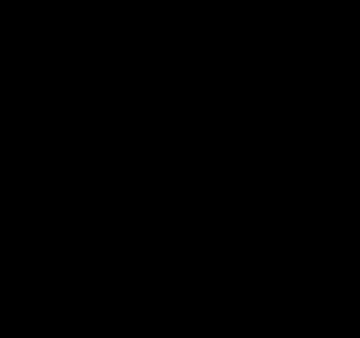
\includegraphics[width=194pt,]{images/lunch.gif}\caption{Tree diagram to enumerate the number of possible lunches.
                \label{lunch}}
\end{figure}

%
\par

 Every path that begins at the position labeled START and goes to the right can be interpreted as a choice of one of the five sandwiches followed by a choice of one of the three beverages. Note that considerable work is required to arrive at the number fifteen this way; but we also get more than just a number. The result is a complete list of all possible lunches. If we need to answer a question that starts with ``How many . . . ,'' enumeration would be done only as a last resort. In a later chapter we will examine more enumeration techniques.
%
\par

 An alternative method of solution for this example is to make the simple observation that there are five different choices for sandwiches and three different choices for beverages, so there are \(5 \cdot 3 = 15\) different lunches that can be ordered.
%
\par

 A listing of possible lunches a person could have is: {(BEEF, milk), (BEEF, juice), (BEEF, coffee), ..., (BOLOGNA, coffee)}.
%
\end{example}
\begin{example}[Counting elements in a cartesion product]\label{cartesian-cardinality}
Let \(A = \{a, b, c, d, e\}\) and \(B = \{1,2,3\}\). From Chapter 1 we know how to list the elements in \(A \times B = \{(a, 1), (a, 2), (a, 3), ..., (e, 3)\}\).  Since the first entry of each pair can be any one of the five elements \(a, b, c, d\), and \(e\), and since the second can be any one of the three numbers 1, 2, and 3, it is quite clear there are 
\(5 \cdot 3 = 15\) different elements in \(A \times B\).
%
\end{example}
\begin{example}[A True-False Questionnaire]\label{questionnaire}
A person is to complete a true-false questionnaire consisting of ten questions. How many different ways are there to answer the questionnaire? Since each question can be answered either of two ways (true or false), and there are a total of ten questions, there are \[ 2 \cdot 2 \cdot 2 \cdot 2 \cdot 2 \cdot 2 \cdot 2 \cdot 2 \cdot 2 \cdot 2 = 2^{10} = 1024\] different ways of answering the questionnaire. The reader is encouraged to visualize the tree diagram of this example, but not to draw it!%
\end{example}
\par

 We formalize the procedures developed in the previous examples with the following rule and its extension.
%
\typeout{************************************************}
\typeout{Subsection 2.1.2 The Rule Of Products:}
\typeout{************************************************}
\subsection[The Rule Of Products:]{The Rule Of Products:}\label{rule-of-products}
If two operations must be performed, and If the first operation can always be performed \(p_1\) different ways and the second operation can always be performed \(p_2\) different ways, then there are \(p_1 p_2\) different ways that the two operations can be performed.
%
\par

Note: It is important that \(p_2\) does not depend on the option that is chosen in the first operation. Another way of saying this is that \(p_2\) is independent of the first operation. If \(p_2\) is dependent on the first operation, then the rule of products does not apply.
%
\begin{example}[Reduced Lunch Possibilities]\label{lunch-possibilites2}
Assume in \hyperref[lunch-possibilies1]{\ref{lunch-possibilies1}}, coffee is not served with a beef or chicken sandwiches. Then by inspection of \hyperref[lunch]{\ref{lunch}} we see that there are only thirteen different choices for lunch. The rule of products does not apply, since the choice of beverage depends on one's choice of a sandwich.%
\end{example}
\par
\emph{Extended Rule Of Products.} The rule of products can be extended to include sequences of more than two operations. If \(n\) operations must be performed, and the number of options for each operation is \(p_1\), \(p_2, \dots, p_n\) respectively, with each \(p_i\)  independent of previous choices, then the \(n\) operations can be performed \(p_1 \cdot p_2 \cdot \cdots \cdot p_n\) different ways.
%
\begin{example}[A Multiple Choice Questionnaire]\label{another_questionnaire}
A questionnaire contains four questions that have two possible answers and three questions with five possible answers. Since the answer to each question is independent of the answers to the other questions, the extended rule of products applies and there are
\(2 \cdot 2 \cdot 2 \cdot 2 \cdot 5 \cdot 5 \cdot 5 = 2^4 \cdot 5^3 = 2000 \) different ways to answer the questionnaire.%
\end{example}
\par

 In Chapter 1 we introduced the power set of a set A, P(A), which is the set of all subsets of A. Can we predict how many elements are in \(\mathcal{P}(A)\) for a given finite set A? The answer is yes, and in fact if \(\lvert A \rvert  = n\), then \(\mathcal{P}(A) = 2^{n}\).  The ease with which we can prove this fact demonstrates the power and usefulness of the rule of products. Do not underestimate the usefulness of simple ideas.
%
\begin{theorem}\label{power-set-cardinality-theorem}
If \(A\) is a finite set, then \(\lvert \mathcal{P}(A) \rvert = 2^{\lvert A \rvert }\)\end{theorem}
\begin{proof}\hypertarget{proof-1}{}

Proof: Consider how we might determine any \(B \in \mathcal{P}(A)\), where \( \lvert A \rvert =n\). For each element \(x \in A\) there are two choices, either \(x \in B\) or \(x \notin B\).  Since there are \(n\)  elements of \(A\)  we have, by the rule of products, 
  \[\underset{n \textrm{ factors}}{\underline{2 \cdot 2 \cdot  \cdots \cdot 2}}=  2^n\]   different subsets of \(A\). Therefore, \(\mathcal{P}(A)= 2^{n}\);
\end{proof}
\typeout{************************************************}
\typeout{Exercises 2.1.3 Exercises}
\typeout{************************************************}
\subsection[Exercises]{Exercises}\label{EXERCISES-FOR-SECTION-2-1}
\hypertarget{exercisegroup-10}{}\begin{exercisegroup}
\item[1.]\hypertarget{exercise-42}{} In horse racing, to bet the ``daily double'' is to select the winners of the first two races of the day. You win only if both selections are correct. In terms of the number of horses that are entered in the first two races, how many different daily double bets could be made?\par\smallskip
\item[2.]\hypertarget{exercise-43}{} Professor Shortcut records his grades using only his students' first and last initials. What is the smallest class size that will definitely force Prof. S. to use a different system?\par\smallskip
\item[3.]\hypertarget{exercise-44}{} A certain shirt comes in four sizes and six colors. One also has the choice of a dragon, an alligator, or no emblem on the pocket. How many different shirts could you order?\par\smallskip
\item[4.]\hypertarget{exercise-45}{} A builder of modular homes would like to impress his potential customers with the variety of styles of his houses. For each house there are blueprints for three different living rooms, four different bedroom configurations, and two different garage styles. In addition, the outside can be finished in cedar shingles or brick. How many different houses can be designed from these plans?\par\smallskip
\item[5.]\hypertarget{exercise-46}{} The Pi Mu Epsilon mathematics honorary society of Outstanding University wishes to have a picture taken of its six officers. There will be two rows of three people. How many different way can the six officers be arranged?\par\smallskip
\item[6.]\hypertarget{exercise-47}{}  An automobile dealer has several options available for each of three different packages of a particular model car: a choice of two styles of seats in three different colors, a choice of four different radios, and five different exteriors. How many choices of automobile does a customer have?\par\smallskip
\item[7.]\hypertarget{exercise-48}{} A clothing manufacturer has put out a mix-and-match collection consisting of two blouses, two pairs of pants, a skirt, and a blazer. How many outfits can you make? Did you consider that the blazer is optional? How many outfits can you make if the manufacturer adds a sweater to the collection?\par\smallskip
\item[8.]\hypertarget{exercise-49}{} As a freshman, suppose you had to take two of four lab science courses, one of two literature courses, two of three math courses, and one of seven physical education courses. Disregarding possible time conflicts, how many different schedules do you have to choose from?\par\smallskip
\item[9.]\hypertarget{exercise-50}{} (a) Suppose each single character stored in a computer uses eight bits. Then each character is represented by a different sequence of eight 0's and l's called a bit pattern. How many different bit patterns are there? (That is, how many different characters could be represented?)
 (b) How many bit patterns are palindromes (the same backwards as forwards)?%
\par
 (c) How many different bit patterns have an even number of 1's?%
\par\smallskip
\item[10.]\hypertarget{exercise-51}{} Automobile license plates in Massachusetts usually consist of three digits followed by three letters. The first digit is never zero. How many different plates of this type could be made?\par\smallskip
\item[11.]\hypertarget{exercise-52}{} (a) Let A = {a, b, c, d}. Determine the number of different subsets of \(A\). 
 (b) Let A = {1, 2, 3, 4, 5}. Determine the number of proper subsets of \(A\) .
%
\par\smallskip
\item[12.]\hypertarget{exercise-53}{} How many integers from 100 to 999 can be written with no 7's?\par\smallskip
\item[13.]\hypertarget{exercise-54}{} Consider three persons, A, B, and C, who are to be seated in a row of three chairs. Suppose A and B are identical twins. How many seating arrangements of these persons can there be
 (a) If you are a total stranger?%
\par
(b) If you are A and B's mother?%
\par
This problem is designed to show you that different people can have different correct answers to the same problem.%
\par\smallskip
\item[14.]\hypertarget{exercise-55}{} How many ways can a student do a ten-question true-false exam if he or she can choose not to answer any number of questions?\par\smallskip
\item[15.]\hypertarget{exercise-56}{} Suppose you have a choice of fish, lamb, or beef for a main course, a choice of peas or carrots for a vegetable, and a choice of pie, cake, or ice cream for dessert. If you must order one item from each category, how many different dinners are possible?%
\par\smallskip
\item[16.]\hypertarget{exercise-57}{} Suppose you have a choice of vanilla, chocolate, or strawberry for ice cream, a choice of peanuts or walnuts for chopped nuts, and a choice of hot fudge or marshmallow for topping. If you must order one item from each category, how many different sundaes are possible?\par\smallskip
\end{exercisegroup}
\par\smallskip\noindent
\hypertarget{exercisegroup-11}{}\begin{exercisegroup}
\item[17.]\hypertarget{exercise-58}{} A questionnaire contains six questions each having yes-no answers. For each yes response, there is a follow-up question with four possible responses.
\leavevmode%
\begin{enumerate}[label=(\alph*)]
\item\hypertarget{li-202}{}
   (a) Draw a tree diagram that illustrates how many ways a single question in the questionnaire can be answered.
\item\hypertarget{li-203}{}
    (b) How many ways can the questionnaire be answered?
\end{enumerate}
\par\smallskip
\item[18.]\hypertarget{exercise-59}{} Ten people are invited to a dinner party. How many ways are there of seating them at a round table? If the ten people consist of five men and five women, how many ways are there of seating them if each man must be surrounded by two women around the table?\par\smallskip
\item[19.]\hypertarget{exercise-60}{} How many ways can you separate a set with \(n\)  elements into two nonempty subsets if the order of the subsets is immaterial? What if the order of the subsets is important?\par\smallskip
\item[20.]\hypertarget{exercise-61}{} A gardener has three flowering shrubs and four nonflowering shrubs. He must plant these shrubs in a row using an alternating pattern, that is, a shrub must be of a different type from that on either side. How many ways can he plant these shrubs? If he has to plant these shrubs in a circle using the same pattern, how many ways can he plant this circle? Note that one nonflowering shrub will be left out at the end.\par\smallskip
\end{exercisegroup}
\par\smallskip\noindent
\typeout{************************************************}
\typeout{Section 2.2 Permutations}
\typeout{************************************************}
\section[Permutations]{Permutations}\label{permutations}

 A number of applications of the rule of products are of a specific type, and because of their frequent appearance they are given their own designation, permutations. Consider the following examples.
%
\begin{example}[Ordering the elements of a set]\label{ordering_a_set}
How many different ways can we order the three different elements of the set \(A = \{a, b, c\}\)? Since we have three choices for position one, two choices for position two, and one choice for the third position, we have, by the rule of products, \(3 \cdot 2 \cdot 1 = 6\) different ways of ordering the three letters. We illustrate through a tree diagram.%
\leavevmode%
\begin{figure}
\centering
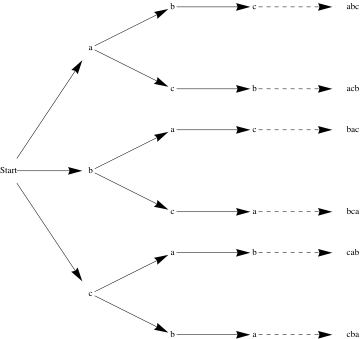
\includegraphics[width=250pt,]{images/tree-of-permutations.svg}\caption{A tree to enumerate permutations of a three element set.
                \label{tree-of-permutations}}
\end{figure}
\par

 Each of the six orderings is called a permutation of the set A.
%
\end{example}
\begin{example}[Ordering a schedule]\label{ordering_a_schedule}
A student is taking five courses in the fall semester. How many different ways can the five courses be listed? There are \(5 \cdot 4 \cdot 3 \cdot 2 \cdot 1 = 120\) different permutations of the set of courses.%
\end{example}
\par

 In each of the above examples of the rule of products we observe that:
\leavevmode%
\begin{enumerate}
\item\hypertarget{li-204}{}
We are asked to order or arrange elements from a single set.\item\hypertarget{li-205}{}
Each element is listed exactly once in each list (permutation). So if there are n choices for position one in a list, there are n - 1 choices for position two, n - 2 choices for position three, etc.\end{enumerate}

%
\begin{example}[Some orderings of a baseball team]\label{some_orderings_of_a_baseball_team}
The alphabetical ordering of the players of a baseball team is one permutation of the set of players. Other orderings of the players' names might be done by batting average, age, or height. The information that determines the ordering is called the key. We would expect that each key would give a different permutation of the names. If there are twenty-five players on the team, there are \(25 \cdot 24 \cdot 23 \cdot \cdots  \cdot 3 \cdot 2 \cdot 1\) different permutations of the players.%
\par
This number of permutations is huge. In fact it is 15511210043330985984000000, but writing it like this isn't all that instructive, while leaving it as a product as we originally had makes it easier to see where the number comes from.  We just need to find a more compact way of writing these products.%
\end{example}
\par

 We now develop notation that will be useful for permutation problems.
%
\begin{definition}[Factorial]\label{Definition-Factorial.}
 If \(n\) is a positive integer then \(n\) factorial is the product of the first \(n\) positive integers and is denoted \(n!\). Additionally, we define zero factorial, \(0!\) to be 1.%
\end{definition}
\label{notation-8}
\par
The first few factorials are 
\[
\begin{array}{ccccccccc}
 \text{n} & 0 & 1 & 2 & 3 & 4 & 5 & 6 &
   7 \\
 \text{n!} & 1 & 1 & 2 & 6 & 24 & 120 &
   720 & 5040 \\
\end{array}
\]%
\par
Note that \(4!\) is 4 times \(3!\), or 24, and \(5!\) is 5 times \(4!\), or 120. In addition, note that as n grows in size, \(n!\) grows extremely quickly. For example, \(11! = 39916800\). If the answer to a problem happens to be \(25!\), as in the previous example, you would never be expected to write that number out completely. However, a problem with an answer of \(\frac{25!}{23!}\) can be reduced to \(25 \cdot 24\), or 600.%
\par

 If \(\lvert A \rvert = n \), there are \(n!\) ways of permuting all \(n\)  elements of \(A\) . We next consider the more general situation where we would like to permute \(k\) elements  out of a set of \(n\)  objects, where \( k \leq n\).
%
\begin{example}[Choosing Club Officers]\label{choosing-club-officers}
A club of twenty-five members will hold an election for president, secretary, and treasurer in that order. Assume a person can hold only one position. How many ways are there of choosing these three officers? By the rule of products there are \(25 \cdot 24 \cdot 23\) ways of making a selection.\end{example}
\begin{definition}[Definition: Permutation]\label{permutation}
 An ordered arrangement of \(k\) elements selected from a set of \(n\) elements, \(0 \leq k \leq  n\), where no two elements of the arrangement are the same, is called a permutation of \(n\) objects taken \(k\) at a time. The total number of such permutations is denoted by \(P(n, k)\).
\end{definition}
\begin{theorem}[Permutation Counting Formula]\label{permutations-counting-formula}
 The number of possible permutations of \(k\)  elements taken from a set of \(n\)  elements is
 \[P(n,k)=n \cdot (n-1) \cdot (n-2) \cdot  \cdots  \cdot (n-k+1) = \prod_{j=0}^{k-1} (n-j) = \frac{n!}{(n-k)!} \]\end{theorem}
\begin{proof}\hypertarget{proof-2}{}
  Case I: If \(k = m\) we have \(P(n,n)=n!=\frac{n!}{(n-n)!}\). %
\par
 Case II: If \(0 \leq  k < n\),then we have \(k\)  positions to fill using \(n\) elements and
\leavevmode%
\begin{enumerate}
\item\hypertarget{li-206}{}
 Position 1 can be filled by any one of \(n-0=n\)  elements
\item\hypertarget{li-207}{}
 Position 2 can be filled by any one of \(n-1\)  elements
\item\hypertarget{li-208}{}
 \( \cdots \)
\item\hypertarget{li-209}{}
 Position k can be filled by any one of \(n-(k-1)=n-k+1\)  elements
\end{enumerate}

%
\par
Hence, by the rule of products, \[P(n;k) = n \cdot(n - 1) \cdot (n - 2) \cdot \cdots \cdot (n - k + 1) = \frac{n!}{(n-k)!}\]. %
\end{proof}
\par

 It is important to note that the derivation of the permutation formula given above was done solely through the rule of products. This serves to reiterate our introductory remarks in this section that permutation problems are really rule-of-products problems.  We close this section with several examples.
%
\begin{example}[Another example of choosing officers]\label{more_club_officers}
A club has eight members eligible to serve as president, vice-president, and treasurer. How many ways are there of choosing these officers?
%
\par

 Solution 1: Using the rule of products. There are eight possible choices for the presidency, seven for the vice-presidency, and six for the office of treasurer. By the rule of products there are \(8 \cdot 7\cdot 6 = 336\) ways of choosing these officers.
%
\par

 Solution 2: Using the permutation formula. We want the total number of permutations of eight objects taken three at a time:
 	\[P(8,3)=\frac{8!}{(8-3)!}=8 \cdot 7 \cdot 6 = 336\]
%
\end{example}
\begin{example}[Course ordering, revisited]\label{course-ordering-revisited}
To count the number of ways to order five courses, we can use the permutation formula. We want the number of permutations of five courses taken five at a time:
\[P(5,5)= \frac{5!}{(5-5)!}= 5!= 120\]\end{example}
\begin{example}[Ordering of digits with and without repeats]\label{ordering-digits}
Consider the digits 1, 2, 3, 4, and 5.
\leavevmode%
\begin{enumerate}
\item\hypertarget{li-210}{} How many three-digit numbers can be formed if no repetition of digits can occur?\item\hypertarget{li-211}{} How many three-digit numbers can be formed if repetition of digits is allowed?\end{enumerate}

%
\par

 Solution to (a): Solution 1: Using the rule of products. We have any one of five choices for digit one, any one of four choices for digit two, and three choices for digit three. Hence, \(5 \cdot 4 \cdot 3 = 60\) different three-digit numbers can be formed.
%
\par
Solution 2; Using the permutation formula. We want the total number of permutations of five digits taken three at a time:
 \[P(5,3)=\frac{5!}{(5-3)!}=5 \cdot 4 \cdot 3 = 60\]%
\par
Solution to (b): The definition of permutation indicates `` ...no two elements in each list are the same.'' Hence the permutation formula cannot be used. However, the rule of products still applies. We have any one of five choices for the first digit, five choices for the second, and five for the third. So there are \(5 \cdot 5\cdot 5 = 125\) possible different three-digit numbers if repetition is allowed.%
\end{example}
\typeout{************************************************}
\typeout{Exercises 2.2.1 Exercises}
\typeout{************************************************}
\subsection[Exercises]{Exercises}\label{exercises-7}
\hypertarget{exercisegroup-12}{}\begin{exercisegroup}
\item[1.]\hypertarget{exercise-62}{} If a raffle has three different prizes and there are 1,000 raffle tickets sold, how many different ways can the prizes be distributed?\par\smallskip
\item[2.]\hypertarget{exercise-63}{} (a) How many three-digit numbers can be formed from the digits 1, 2, 3 if no repetition of digits is allowed? List the three-digit numbers.
 (b) How many two-digit numbers can be formed if no repetition of digits is allowed? List them.%
\par
 (c) How many two-digit numbers can be obtained if repetition is allowed?%
\par\smallskip
\item[3.]\hypertarget{exercise-64}{} How many eight-letter words can be formed from the 26 letters in the alphabet? Even without concerning ourselves about whether the words make sense, there are two interpretations of this problem. Answer both.\par\smallskip
\item[4.]\hypertarget{exercise-65}{} Let A be a set with \( \lvert A \rvert = n \).
Determine 
\leavevmode%
\begin{enumerate}[label=(\alph*)]
\item\hypertarget{li-212}{}\( \lvert A^3 \rvert \)\item\hypertarget{li-213}{}\( \lvert \{ ( a, b, c) \mid \textrm{ each coordinate is different} \} \rvert \)\end{enumerate}

%
\par\smallskip
\item[5.]\hypertarget{exercise-66}{} The state finals of a high school track meet involves fifteen schools. How many ways can these schools be listed in the program?\par\smallskip
\item[6.]\hypertarget{exercise-67}{} Consider the three-digit numbers that can be formed from the digits 1, 2, 3, 4, and 5 with no repetition of digits allowed.%
\par
a. How many of these are even numbers?%
\par
b. How many are greater than 250?%
\par\smallskip
\item[7.]\hypertarget{exercise-68}{}a. How many ways can the coach at Tall U. fill the five starting positions on a basketball team if each of his 15 players can play any position?%
\par
b. What is the answer if the center must be one of two players?%
\par\smallskip
\item[8.]\hypertarget{exercise-69}{}\leavevmode%
\begin{enumerate}[label=(\alph*)]
\item\hypertarget{li-214}{}How many ways can a gardener plant five different species of shrubs in a circle?\item\hypertarget{li-215}{}What is the answer if two of the shrubs are the same?\item\hypertarget{li-216}{}What is the answer if all the shrubs are identical?\end{enumerate}
\par\smallskip
\item[9.]\hypertarget{exercise-70}{} The president of the Math and Computer Club would like to arrange a meeting with six attendees, the president included. There will be three computer science majors and three math majors at the meeting. How many ways can the six people be seated at a circular table if the president does not want people with the same majors to sit next to one other?\par\smallskip
\end{exercisegroup}
\par\smallskip\noindent
\hypertarget{exercisegroup-13}{}\begin{exercisegroup}
\item[10.]\hypertarget{exercise-71}{} Six people apply for three identical jobs and all are qualified for the positions. Two will work in New York and the other one will work in San Diego. How many ways can the positions be filled?\par\smallskip
\item[11.]\hypertarget{exercise-72}{}
 Let \(A = \{1, 2, 3, 4\} \). Determine the cardinality of
 \leavevmode%
\begin{enumerate}[label=(\alph*)]
\item\hypertarget{li-217}{}\(\{ (a_1,a_2) \mid a_1 \neq a_2 \}\)\item\hypertarget{li-218}{}What is the answer to the previous part if \(\lvert A \rvert = n\)\item\hypertarget{li-219}{}If \(\lvert A \rvert =n\), determine the number of \(m\)-tuples in \(A\), \(m \leq n\), where each coordinate is different from the other coordinates.\end{enumerate}
\par\smallskip
\end{exercisegroup}
\par\smallskip\noindent
\typeout{************************************************}
\typeout{Section 2.3 Partitions of Sets and the Law of Addition}
\typeout{************************************************}
\section[Partitions of Sets and the Law of Addition]{Partitions of Sets and the Law of Addition}\label{Partitions-and-Law-of-Addition}

 One way of counting the number of students in your class would be to count the number in each row and to add these totals. Of course this problem is simple because there are no duplications, no person is sitting in two different rows. The basic counting technique that you used involves an extremely important first step, namely that of partitioning a set. The concept of a partition must be clearly understood before we proceed further.
%
\begin{definition}[Definition: Partition.]\label{partition}
 A partition of set \(A\) is a set of one or more nonempty subsets of \(A\): \(A_1, A_2, A_3, \cdots\), such that every element of \(A\) is in exactly one set.  Symbolically, 
\leavevmode%
\begin{enumerate}
\item\hypertarget{li-220}{}\(A_1 \cup A_2 \cup A_3 \cup \cdots = A\)\item\hypertarget{li-221}{}If  \(i \neq j\) then \(A_i \cap A_j = \emptyset\)\end{enumerate}
\end{definition}
\par

 The subsets in a partition are often referred to as blocks. Note how our definition allows us to partition infinite sets, and to partition a set into an infinite number of subsets. Of course, if \(A\)  is finite the number of subsets can be no larger than \(\lvert A \rvert \).
%
\begin{example}[Some partitions of a four element set]\label{some-partitions-4}

  Let \(A = \{a, b, c, d\}\). Examples of partitions of \(A\)  are:
\leavevmode%
\begin{itemize}[label=\textbullet]
\item{} \(\{\{a\}, \{b\}, \{c, d\}\}\)\item{} \(\{\{a, b\}, \{c, d\}\}\)\item{} \(\{\{a\}, \{b\}, \{c\}, \{d\}\}\)\end{itemize}
How many others are there, do you suppose?
%
\par
There are 15 different partitions.  The most efficient way to count them all is to classify them by the size of blocks.   For example, the partition \(\{\{a\}, \{b\}, \{c, d\}\}\) has block sizes 1, 1, and 2.
%
\end{example}
\begin{example}[Some Integer Partitions]\label{some-integer-partitions}
Two examples of partitions of set of integers \(\mathbb{Z}\) are 
\leavevmode%
\begin{itemize}[label=\textbullet]
\item{}\(\{\{n\} \mid n \in \mathbb{Z}\}\) and\item{} \(\{\{ n \in \mathbb{Z} \mid n < 0\}, \{0\},\{ n \in \mathbb{Z} \mid 0 < 0 \}\}\).\end{itemize}
%
\par
 The set of subsets \(\{\{n \in \mathbb{Z} \mid n \geq 0\},\{n \in \mathbb{Z} \mid  n \leq 0\}\}\) is not a partition because the two subsets have a nonempty intersection. A second example of a non-partition is 
\(\{\{n \in \mathbb{Z} \mid  \lvert n \rvert = k\} \mid k = -1, 0, 1, 2, \cdots\}\) because one of the blocks, when \(k=-1\) is empty.%
\end{example}
\par
One could also think of the concept of partitioning a set as a ``packaging problem.'' How can one ``package'' a carton of, say, twenty-four cans? We could use: four six-packs, three eight-packs, two twelve-packs, etc. In all cases: (a) the sum of all cans in all packs must be twenty-four, and (b) a can must be in one and only one pack.
%
\typeout{************************************************}
\typeout{Subsection 2.3.1 The Basic Law Of Addition:}
\typeout{************************************************}
\subsection[The Basic Law Of Addition:]{The Basic Law Of Addition:}\label{basic-law-addition}
If \(A\) is a finite set, and if \(\{A_1,A_2,\ldots ,A_n\}\) is a partition of \(A\) , then 
\[\lvert A \rvert = \lvert A_1 \rvert + \lvert A_2 \rvert + \cdots + \lvert A_n \rvert = \sum _{k=1}^n  \lvert A_k \rvert\]
%
\par

 The basic law of addition can be rephrased as follows: If \(A\)  is a finite set where \(A_1 \cup A_2 \cup \cdots \cup A_n = A\) and where \(A_i \cap A_j\) whenever \(i \neq j\), then
 \[\lvert A \rvert = \lvert A_1 \cup A_2 \cup  \cdots \cup A_n  \rvert = \lvert A_1 \rvert + \lvert A_2 \rvert + \cdots + \lvert A_n \rvert \]
%
\begin{example}[Counting All Students]\label{counting-all-students}
The number of students in a class could be determined by adding the numbers of students who are freshmen, sophomores, juniors, and seniors, and those who belong to none of these categories. However, you probably couldn't add the students by major, since some students may have double majors.
%
\end{example}
\begin{example}[Counting Students in Disjoint Classes.]\label{student-counting-disjoint}
The sophomore computer science majors were told they must take one and only one of the following courses, Cryptography, Data Structures, or Javascript, in a given semester. The numbers in each course, respectively, for sophomore CS majors, were 75, 60, 55. How many sophomore C.S. majors are there? The Law of Addition applies here. There are exactly \(75 + 60 + 55 = 190\) CS majors since the rosters of the three courses listed above would be a partition of the CS majors.%
\end{example}
\begin{example}[Counting Students in Non-disjoint Classes]\label{student-counting-nondisjoint}
It was determined that all junior computer science majors take at least one of the following courses: Algorithms, Logic Design, and Compiler Construction. Assume the number in each course was was 75, 60 and 55, respectively for the three courses listed. Further investigation indicated ten juniors took all three courses, twenty-five took  Algorithms and Logic Design, twelve took Algorithms and Compiler Construction, and fifteen took Logic Design and Compiler Construction. How many junior C.S. majors are there?
%
\par
\hyperref[student-counting-disjoint]{\ref{student-counting-disjoint}} was a simple application of the law of addition, however in this example some students are taking two or more courses, so a simple application of the law of addition would lead to double or triple counting. We rephrase information in the language of sets to describe the situation more explicitly.
%
\par

 \(A\) = the set of all junior computer science majors
%
\par

  \(A_1\) = the set of all junior computer science majors who took Algorithms
%
\par

  \(A_2\) = the set of all junior computer science majors who took Logic Design
%
\par

  \(A_3\) = the set of all junior computer science majors who took Compiler Construction
%
\par

 Since all sophomore CS majors must take at least one of the courses, the number we want is:
 \[\lvert A \rvert = \lvert A_1 \cup A_2 \cup A_3 \rvert = \lvert A_1 \rvert + \lvert A_2 \rvert + \lvert A_3 \rvert - \textrm{repeats}.\]
%
\par

 A Venn diagram is helpful to visualize the problem. In this case the universal set \(U\)  can stand for 	all students in the university.
%
\leavevmode%
\begin{figure}
\centering
\IfFileExists{images/sageplot-venn-CS_Students.pdf}%
{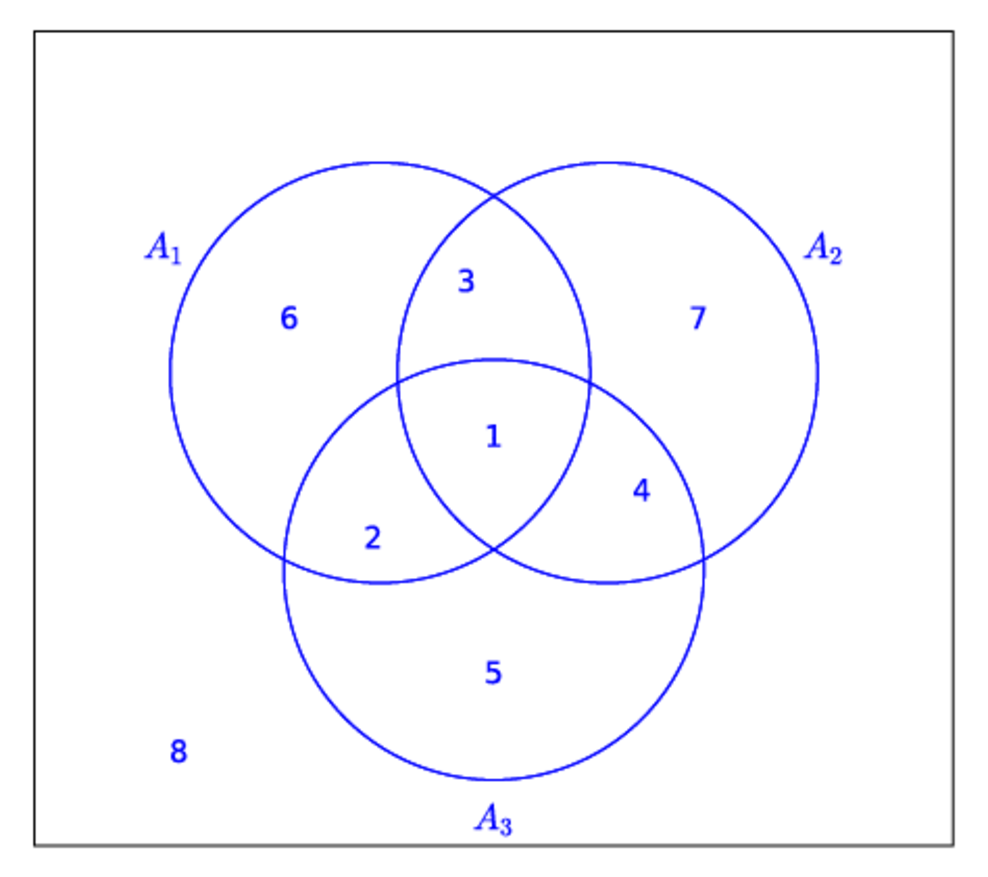
\includegraphics[width=0.80\textwidth]{images/sageplot-venn-CS_Students.pdf}}%
{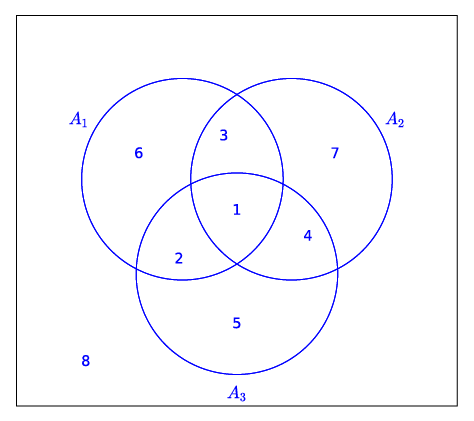
\includegraphics[width=0.80\textwidth]{images/sageplot-venn-CS_Students.png}}
\caption{Venn Diagram\label{venn_diagram_CS_Students}}
\end{figure}
\par

 We see that the whole universal set is naturally partitioned into subsets that are labeled by the numbers 1 through 8, and the set \(A\)  is  partitioned into subsets labeled 1 through 7. The region labeled 8 represents all students who are not junior CS majors.  Note also that students in the subsets labeled 2, 3, and 4 are double counted, and those in the subset labeled 1 are triple counted. To adjust, we must subtract the numbers in regions 2, 3 and 4.  This can be done by subtracting the numbers in the intersections of each pair of sets.  However, the individuals in region 1 will have been removed three times, just as they had been originally added three times.  Therefore, we must finally add their number back in.
%
\par
\[\begin{split}
 \lvert A \rvert & =  \lvert A_1 \cup A_2 \cup A_3 \rvert \\ 
 & = \lvert A_1 \rvert + \lvert A_2 \rvert + \lvert A_3 \rvert - \textrm{repeats} \\
 & = \lvert A_1 \rvert + \lvert A_2 \rvert + \lvert A_3 \rvert - \textrm{duplicates} + \textrm{triplicates}  \\
 & = \lvert A_1 \rvert + \lvert A_2 \rvert + \lvert A_3 \rvert - (\lvert A_1 \cap A_2 \rvert + \lvert A_1 \cap A_3 \rvert+ \lvert A_2 \cap A_3 \rvert) + \lvert A_1 \cap A_2 \cap A_3 \rvert  \\
 & = 75 + 60 + 55 - 25 - 12 - 15 + 10 = 148 \\
\end{split}
\]
%
\end{example}
\par

The ideas used in this latest example gives rise to a basic counting technique:
%
\typeout{************************************************}
\typeout{Subsection 2.3.2 Laws of Inclusion-Exclusion}
\typeout{************************************************}
\subsection[Laws of Inclusion-Exclusion]{Laws of Inclusion-Exclusion}\label{inclusion-exclusion}
Given finite sets \(A_1, A_2, A_3\), then
\leavevmode%
\begin{enumerate}
\item\hypertarget{li-227}{}\( \lvert A_1 \cup A_2 \rvert =\lvert A_1 \rvert + \lvert A_2 \rvert - \lvert A_1 \cap A_2 \rvert  \)\item\hypertarget{li-228}{}\(  \lvert A_1 \cup A_2 \cup A_3 \rvert =\lvert A_1 \rvert + \lvert A_2 \rvert + \lvert A_3 \rvert - (\lvert A_1 \cap A_2 \rvert + \lvert A_1 \cap A_3 \rvert+ \lvert A_2 \cap A_3 \rvert) + \lvert A_1 \cap A_2 \cap A_3 \rvert \)\end{enumerate}
 
%
\par
The inclusion-exclusion laws extend to more than three sets, as will be explored in the exercises.%
\par

 In this section we saw that being able to partition a set into disjoint subsets gives rise to a handy counting technique. Given a set, there are many ways to partition depending on what one would wish to accomplish. One natural partitioning of sets is apparent when one draws a Venn diagram. This particular partitioning of a set will be discussed further in Chapters 4 and 13.
%
\typeout{************************************************}
\typeout{Exercises 2.3.3 Exercises for Section 2.3}
\typeout{************************************************}
\subsection[Exercises for Section 2.3]{Exercises for Section 2.3}\label{exercises-2-3}
\hypertarget{exercisegroup-14}{}\begin{exercisegroup}
\item[1.]\hypertarget{exercise-73}{} List all partitions of the set \(A =\{a, b, c\}\).
 \par\smallskip
\item[2.]\hypertarget{exercise-74}{}Which of the following collections of subsets of the plane, \( \mathbb{R}^2\), are partitions?
\leavevmode%
\begin{enumerate}[label=(\alph*)]
\item\hypertarget{li-229}{}\( \{ \{(x, y) \mid x + y = c \} \mid c \in \mathbb{R} \}\)\item\hypertarget{li-230}{} The set of all circles in \( \mathbb{R}^2 \)\item\hypertarget{li-231}{} The set of all circles in \(\mathbb{R}^2\) centered at the origin together with the set \(\{(0,0)\}\)\item\hypertarget{li-232}{}\(\{\{(x, y)\} \mid (x, y) \in \mathbb{R}^2  \} \)\end{enumerate}
\par\smallskip
\item[3.]\hypertarget{exercise-75}{}A student, on an exam paper, defined the term partition the following way: "Let \(A\)  be a set. A partition of \(A\) is any set of nonempty subsets \(A_1, A_2, A_3, \dots\)  of \(A\) such that each element of A is in one of the subsets."  Is this definition correct? Why?
\par\smallskip
\item[4.]\hypertarget{exercise-76}{} Let \(A_1\) and \(A_2\) be subsets of a set \(U\).   Draw a Venn diagram of this situation and shade in the subsets \(A_1 \cap A_2\), \(A_1^c \cap A_2\),\(A_1 \cap A_2^c\),and \(A_1^c \cap A_2^c\) . Use the resulting diagram and the definition of partition to convince yourself that the subset of these four subsets that are nonempty form a partition of \(U\).
\par\smallskip
\item[5.]\hypertarget{exercise-77}{} Show that \(\{\{2 n | n \in \mathbb{Z}\}, \{2 n + 1 | n \in \mathbb{Z}\}\}\) is a partition of \(\mathbb{Z}\). Describe this partition using only words.\par\smallskip
\item[6.]\hypertarget{exercise-78}{} (a) A group of 30 students were surveyed and it was found that 18 of them took Calculus and 12 took Physics. If all students took at least one course, how many took both Calculus and Physics? Illustrate using a Venn diagram.\\
 (b) What is the answer to the question in part (a) if five students did not take either of the two courses? Illustrate using a Venn diagram.
\par\smallskip
\item[7.]\hypertarget{exercise-79}{}A survey of 90 people, 47 of them played tennis and 42 of them swam. If 17 of the them participated in both activities, how many of them participated in neither.%
\par\smallskip
\item[8.]\hypertarget{exercise-80}{}A survey of 300 people found that 60 owned an iPhone 75 owned an Blackberry, and 30 owned an Android phone. Furthermore, 40 owned both an iPhone and Blackberry, 12 owned both an iPhone and Android phone, and 8 owned a Blackberry and an Android phone. Finally, 3 owned all three phones.%
\leavevmode%
\begin{enumerate}[label=(\alph*)]
\item\hypertarget{li-233}{} How many people surveyed owned none of the three phones?\item\hypertarget{li-234}{} How many people owned an Blackberry but not an iPhone?\item\hypertarget{li-235}{} How many owned a Blackberry but not an Android?\end{enumerate}
\par\smallskip
\end{exercisegroup}
\par\smallskip\noindent
\hypertarget{exercisegroup-15}{}\begin{exercisegroup}
\item[9.]\hypertarget{exercise-81}{}\leavevmode%
\begin{enumerate}[label=(\alph*)]
\item\hypertarget{li-236}{} Use Inclusion-exclusion Law 1 to derive Law 2. Note: a knowledge of basic set laws is needed for this exercise.\item\hypertarget{li-237}{} State and derive the Inclusion-exclusion law for four sets.\end{enumerate}
\par\smallskip
\item[10.]\hypertarget{exercise-82}{} To complete your spring schedule, you must add Calculus and Physics. At 9:30, there are three Calculus sections and two Physics sections; while at 11:30, there are two Calculus sections and three Physics sections.  How many ways can you complete your schedule if your only open periods are 9:30 and 11:30?\par\smallskip
\end{exercisegroup}
\par\smallskip\noindent
\hypertarget{exercisegroup-16}{}\begin{exercisegroup}
\item[11.]\hypertarget{exercise-83}{}The definition of \(\mathbb{Q}  = \{a/b \mid a, b \in \mathbb{Z}, b \neq 0\}\) given in Chapter 1 is  awkward. If we use the definition to list elements in \(\mathbb{Q}\), we will have duplications such as \(\frac{1}{2}\), \(\frac{-2}{-4}\) and \(\frac{300}{600}\)   Try to write a more precise definition of the rational numbers so that there is no duplication of elements.
\par\smallskip
\end{exercisegroup}
\par\smallskip\noindent
\typeout{************************************************}
\typeout{Section 2.4 Combinations and the Binomial Theorem}
\typeout{************************************************}
\section[Combinations and the Binomial Theorem]{Combinations and the Binomial Theorem}\label{combinations-and-the-binomial-theorem}
\typeout{************************************************}
\typeout{Subsection 2.4.1 Combinations}
\typeout{************************************************}
\subsection[Combinations]{Combinations}\label{combinations}
 In Section 2.1 we investigated the most basic concept in combinatorics, namely, the rule of products. Even though in this section we investigate other counting formulas, it is of paramount importance to keep this fundamental process in mind. In Section 2.2 we saw that a subclass of rule-of-products problems appears so frequently that we gave them a special designation, namely, permutations, and we derived a formula as a computational aid to assist us. In this section we will investigate another counting formula that are used to count combinations, which are subsets of a certain size..%
\par
In many rule-of-products applications the permutation or order is important, as in the situation of the order of putting on one's socks and shoes; in some cases it is not important, as in placing coins in a vending machine or in the listing of the elements of a set. Order is important in permutations. Order is not important in combinations.%
\begin{example}[Counting Permutations]\label{counting-permuations-multiple-ways}
How many different ways are there to permute three letters from the set \(A = \{a, b, c, d\}\)?  From the \hyperref[permutations-counting-formula]{Permutation Counting Formula} there are \(P(4,3)=\frac{4!}{(4-3)!} = 24\) different orderings of three letters from \(A\)\end{example}
\begin{example}[Counting with No Order]\label{four-choose-three}
How many ways can we select a set of three letters from  \(A = \{a, b, c, d\}\)?  Note here that we are not concerned with the order of the three letters. By trial and error, abc, abd, acd, and bcd are the only listings possible. To repeat, we were looking for all three-element subsets of the set A. Order is not important in sets. The notation for choosing 3 elements from 4 is most commonly \(\binom{4}{3}\) or occasionally \(C(4,3)\), either of which is read ``4 choose 3'' or the number of combinations for four objects taken three at a time.\end{example}
\begin{definition}[Binomial Coefficient]\label{binomial-coefficient}
Let \(n\) and \(k\) be nonnegative integers.  The binomial coefficient \(\binom{n}{k}\) represents the number of combinations of \(n\) objects taken \(k\) at a time, and is read ``\(n\) choose \(k\).''%
\end{definition}
\label{notation-9}
\par
We would now like to investigate the relationship between permutation and combination problems in order to derive a formula for \(\binom{n}{k}\)%
\par
Let us reconsider the \hyperref[four-choose-three]{Counting with No Order}. There are \(3 ! = 6\) different orderings for each of the three-element subsets. The table below lists each subset of \(A\)  and all permutations of each subset on the same line.
\[
 \begin{array}{cc}
 \textrm{subset} & \textrm{permutations} \\
 abc & abc,acb,bca,bac,cab,cba \\
 abd & abd,adb,bda,bad,dab,dba \\
 acd & acd,adc,cda,cad,dac,dca \\
 bcd & bcd,bdc,cdb,cbd,dbc,dcb \\
\end{array}
 \]%
\par
 Hence, \(\binom{4}{3} = \frac{P(4,3)}{3!} = \frac{4!}{(4-3)! \cdot 3!} = 4\)%
\par
 We generalize this result in the following theorem:%
\begin{theorem}[Binomial Coefficient Formula]\label{binomial-coefficient-formula}

If \(n\) and \(k\) are nonnegative integers with \(0 \leq k \leq n\), then the number \(k\)-element subsets of an \(n\) element set is equal to \[\binom{n}{k} = \frac{n!}{(n-k)! \cdot k!} \]\end{theorem}
\begin{proof}\hypertarget{proof-3}{}
Proof 1: There are \(k!\) ways of ordering the elements of any \(k\) element set.Therefore,
\[\binom{n}{k} = \frac{P(n,k)}{k!} = \frac{n!}{(n-k)! k!}.\]%
\par
Proof 2: To ``construct'' a permutation of \(k\)  objects from a set of \(n\) elements, we can first choose one of the subsets of objects and second, choose one of the \(k!\)  permutations of those objects. By the rule of products,\[P(n,k) = \binom{n}{k} \cdot k!\] and solving for \(\binom{n}{k}\) we get the desired formula.%
\end{proof}
\begin{example}[Flipping Coins]\label{flipping-coins}
  Assume an evenly balanced coin is tossed five times. In how many ways can three heads be obtained? This is a combination problem, because the order in which the heads appear does not matter. The number of ways to get three heads is \(\binom{5}{3}= \frac{5 \cdot 4}{2 \cdot 1} = 10\).
%
\end{example}
\begin{example}[Listing Five Flips, taking order into account]\label{five-flips}
Determine the total number of ways a fair coin can land if tossed five consecutive times. The five tosses can produce any one of the following mutually exclusive, disjoint events: 5 heads, 4 heads, 3 heads, 2 heads, 1 head, or 0 heads. Hence by the law of addition we have:
\[\binom{5}{5}+\binom{5}{4}+\binom{5}{3}+\binom{5}{2}+\binom{5}{1}+\binom{5}{0}= 1 + 5 +10+10+5+1 = 32\] ways to observe the five flips%
\par
 Of course, we could also have applied the extended rule of products, and since there are two possible outcomes for each of the five tosses, we have \(2^5 = 32\) ways.%
\end{example}
\par
You might think that counting something two ways is a waste of time but solving a problem two different ways often is instructive and leads to valuable insights. In this case, it suggests a general formula for the sum 
\(\sum_{k=0}^n \binom{n}{k}\). In the case of \(n = 5\), we get \(2^5\) so it is reasonable to expect that the general sum is \(2^n\), and it is.%
\begin{example}[A Committee of Five]\label{committee-of-five}
A committee usually starts as an unstructured set of people selected from a larger membership. Therefore, a committee can be thought of as a combination. If a club of 25 members has a five-member social committee, there are \(\binom{25}{5}=\frac{25 24 23 22 21}{5!} = 53130\) different possible social committees. If any structure or restriction is placed on the way the social committee is to be selected, the number of possible committees will probably change. For example, if the club has a rule that the treasurer must be on the social committee, then the number of possibilities is reduced to \(\binom{24}{4}=\frac{24 23 22 21}{4!} = 10626\). %
\par
 If we further require that a chairperson other than the treasurer be selected for the social committee, we have  \(\binom{24}{4} \cdot 4 = 42504\) different possible social committees. The choice of the four non-treasurers accounts for the factor \(\binom{24}{4}\) while the need to choose a chairperson accounts for the 4.%
\end{example}
\begin{example}[Binomial Coefficients - Extreme Cases]\label{extreme-binomial-cases}
By simply applying the definition of a \hyperref[binomial-coefficient]{Binomial Coefficient} as a number of subsets we see that there is \(\binom{n}{0} = 1\) way of choosing a combination of zero elements from a set of \(n\). In addition, we see that   there is \(\binom{n}{n} = 1\) way of choosing a combination of \(n\) elements from a set of \(n\). %
\par
We could compute these values using the formula we have developed, but no arithmetic is really needed here.  Other properties of binomial coefficients that can be derived using the subset definition will be seen in the exercises%
\end{example}
\typeout{************************************************}
\typeout{Subsection 2.4.2 The Binomial Theorem}
\typeout{************************************************}
\subsection[The Binomial Theorem]{The Binomial Theorem}\label{the-binomial-theorem}

 The binomial theorem gives us a formula for expanding \(\( x + y \)^{n}\), where \(n\)  is a nonnegative integer. The coefficients of this expansion are precisely the binomial coefficients that we have used to count combinations. Using high school algebra we can  expand the expression for integers from 0 to 5:
\leavevmode%
\begin{table}
\centering
Pascal's Triangle \[
 \begin{array}{cc}
 n & (x + y)^n \\
 0 & 1 \\
 1 & x+y \\
 2 & x^2+2 x y+y^2 \\
 3 & x^3+3 x^2 y+3 x y^2+y^3 \\
 4 & x^4+4 x^3 y+6 x^2 y^2+4 x y^3+y^4
   \\
 5 & x^5+5 x^4 y+10 x^3 y^2+10 x^2
   y^3+5 x y^4+y^5 \\
\end{array}
 \]
 
 

 
 \end{table}
%
\par
In the expansion of \(( x + y )^{5} \)  we note that the coefficient of the third term is \(\binom{5}{3} = 10\), and that of the sixth term is  \(\binom{5}{5}=1\). We can rewrite the expansion as 
\[\binom{5}{0} x^5+\binom{5}{1} x^4 y+\binom{5}{2} x^3 y^2+\binom{5}{3} x^2 y^3+\binom{5}{4} x y^4+ \binom{5}{5} y^5
\]%
\par

 In summary, in the expansion of \(( x + y )^{n}\) we note:
\leavevmode%
\begin{enumerate}
\item\hypertarget{li-238}{}The first term is \(x^n\) and the last term is \(y^n\). \item\hypertarget{li-239}{} With each successive term, exponents of \(x\) decrease by 1 as those of \(y\) increase by 1. For any term the sum of the exponents is \(n\).\item\hypertarget{li-240}{}  The coefficient of \(x^{n-k} y^k\) is \(\binom{n}{k}\).\item\hypertarget{li-241}{} The triangular array of numbers in \hyperref[pascal]{} is called Pascal's triangle after the seventeenth-century French mathematician Blaise Pascal. Note that each number in the triangle other than the 1's at the ends of each row is the sum of the two numbers to the right and left of it in the row above.\end{enumerate}

%
\begin{theorem}[The Binomial Theorem]\label{binomial-theorem}
 If \(n \geq  0\), and \(x\) and \(y\) are numbers, then
\[(x+y)^{n} = \sum_{k=0}^n \binom{n}{k} x^{n-k} y^k\]\end{theorem}
\begin{proof}\hypertarget{proof-4}{}
This theorem will proven using a procedure called mathematical induction, which will be introduced in Chapter 3. \end{proof}
\begin{example}[Identifying a term in an expansion]\label{term-in-an-expansion}
Find the third term in the expansion of \(( x-y )^{4}\). The third term,  when \(k=2\), is \(\binom{4}{2} x^{4-2} y^2 = 6 x^2 y^2\).%
\end{example}
\begin{example}[A Binomial Expansion]\label{a-full-expansion}

Expand \((3 x - 2 )^{3}\).  If we replace \(x\)  and \(y\)  in the Binomial Theorem with \(3x\) and \(-2\), respectively, we get
\[\begin{split} 
\sum_{k=0}^3 \binom{3}{k} (3x)^{n-k} (-2)^k & = \binom{3}{0} (3x)^{3} (-2)^0 + \binom{3}{1} (3x)^{2} (-2)^1 + \binom{3}{2} (3x)^{1} (-2)^2 + \binom{3}{3} (3x)^{0} (-2)^3 \\
& = 27 x^3 - 54 x^2 + 36 x - 8 \\
\end{split}
\]\end{example}
\typeout{************************************************}
\typeout{Subsection 2.4.3  \emph{Mathematica}  Note}
\typeout{************************************************}
\subsection[ \emph{Mathematica}  Note]{ \emph{Mathematica}  Note}\label{mathematica-binomial}
\emph{Mathematica}  has a built-in function for binomial coefficients, \(\texttt{Binomial}\). Unlike the examples we've concentrated on that can be done without technology, you can compute extremely large values. For 
example, a bridge hand is a 13 element subset of a standard 52 card deck. The order in which the cards come to the player doesn't matter. From the point of view of a single player, the number of possible bridge hands is \(\texttt{Binomial[52,13]}\), which is easily computed with \(Mathematica\) with an output of 635013559600%
\par
In bridge, the location of a hand in relation to the dealer has some bearing on the game. An even truer indication of the number of possible hands takes into account \(each\)  player's possible hand. It is customary 
to refer to bridge positions as West, North, East and South. We can apply the rule of product to get the total number of bridge hands with the following logic. West can get any of the \(\binom{52}{13}\) hands identified above. Then North get 13 of the remaining 39 cards and so has  \(\binom{39}{13}\) possible hands. East then gets 13 of the 26 remaining cards, which has \(\binom{26}{13}\)  possibilities. South gets the remaining cards. Therefore the number of bridge hands is computed by evaluating the expression \[\texttt{Binomial[52,13] Binomial[52,13] Binomial[52,13]}\] which is equal to 53644737765488792839237440000%
\typeout{************************************************}
\typeout{Subsection 2.4.4 Sage Note}
\typeout{************************************************}
\subsection[Sage Note]{Sage Note}\label{sage-bridge-hands}

 Sage will do the same calculations for bridge hands just as easily. A correct input is provided in the sage cell below.  Click on the evaluate button to see the output.
%
\begin{lstlisting}[style=sageinput]
binomial(52,13)*binomial(39,13)*binomial(26,13)
\end{lstlisting}
\typeout{************************************************}
\typeout{Exercises 2.4.5 Exercises}
\typeout{************************************************}
\subsection[Exercises]{Exercises}\label{exercises-2-4}
\hypertarget{exercisegroup-17}{}\begin{exercisegroup}
\item[1.]\hypertarget{exercise-84}{} The judiciary committee at a college is made up of three faculty members and four students. If ten faculty members and 25 students have been nominated for the committee, how many judiciary committees could be formed at this point	?\par\smallskip
\item[2.]\hypertarget{exercise-85}{} Suppose that a single character is stored in a computer using eight bits.%
\par
a. How many bit patterns have exactly three 1 's?%
\par
b. How many bit patterns have at least two 1 's?%
\par\smallskip
\item[3.]\hypertarget{exercise-86}{} How many subsets of \(\{1, 2, 3, \dots , 10\}\) contain at least seven elements?\par\smallskip
\item[4.]\hypertarget{exercise-87}{} The congressional committees on mathematics and computer science are made up of five congressmen each, and a congressional rule is that the two committees must be disjoint. If there are 385 members of congress, how many ways could the committees be selected?
  \par\smallskip
\item[5.]\hypertarget{exercise-88}{}Expand \( ( 2x - 3y )^4\)\par\smallskip
\item[6.]\hypertarget{exercise-89}{}Find the fourth term of the expansion of \((x -2y)^6\).\par\smallskip
\item[7.]\hypertarget{exercise-90}{}(a) A poker game is played with 52 cards. How many ``hands'' of five cards are possible?%
\par
(b) If there are four people playing, how many five-card ``hands'' are possible on the first deal?%
\par\smallskip
\item[8.]\hypertarget{exercise-91}{} A flush in a five-card poker hand is five cards of the same suit. How many spade flushes are possible in a 52-card deck? How many flushes are possible in any suit?\par\smallskip
\item[9.]\hypertarget{exercise-92}{} How many five-card poker hands using 52 cards contain exactly two aces?\par\smallskip
\item[10.]\hypertarget{exercise-93}{}  In poker, a full house is three-of-a-kind and a pair in one hand; for example, three fives and two queens. How many full houses are possible from a 52- card deck?\par\smallskip
\item[11.]\hypertarget{exercise-94}{} A class of twelve computer science students are to be divided into three groups of 3, 4, and 5 students to work on a project. How many ways can this be done if every student is to be in exactly one group?\par\smallskip
\end{exercisegroup}
\par\smallskip\noindent
\hypertarget{exercisegroup-18}{}\begin{exercisegroup}
\item[12.]\hypertarget{exercise-95}{} Explain in words why the following equalities are true based on number of subsets,  and then verify the equalities using the formula for binomial coefficients.
\leavevmode%
\begin{enumerate}[label=(\alph*)]
\item\hypertarget{li-242}{}\(\binom{n}{1} = n\) \item\hypertarget{li-243}{}\(\binom{n}{k} = \binom{n}{n-k}\), \( 0 \leq k \leq n\)\end{enumerate}
\par\smallskip
\item[13.]\hypertarget{exercise-96}{}  There are ten points, \(P_1, P_2, \dots , P_{10}\) on a plane, no three on the same line.%
\leavevmode%
\begin{enumerate}[label=(\alph*)]
\item\hypertarget{li-244}{}How many lines are determined by the points?\item\hypertarget{li-245}{} How many triangles are determined by the points?\end{enumerate}
\par\smallskip
\item[14.]\hypertarget{exercise-97}{} How many ways can \(n\)  persons be grouped into pairs when \(n\)  is even? Assume the order of the pairs matters, but not the order within the pairs. For example, if \(n=4\), the six different groupings would be
\[\begin{array}{cc}
 \{1,2\} & \{3,4\} \\
 \{1,3\} & \{2,4\} \\
 \{1,4\} & \{2,3\} \\
 \{2,3\} & \{1,4\} \\
 \{2,4\} & \{1,3\} \\
 \{3,4\} & \{1,2\} \\
\end{array}
\]\par\smallskip
\item[15.]\hypertarget{exercise-98}{} Use the binomial theorem to prove that if \(A\) is a finite set, then 
\(\mathscr{P}(A) = 2^{\lvert A \rvert}\)\par\smallskip
\item[16.]\hypertarget{exercise-99}{}\leavevmode%
\begin{enumerate}[label=(\alph*)]
\item\hypertarget{li-246}{}A state's lottery involves choosing six different numbers out of a possible 36. How many ways can a person choose six numbers?\item\hypertarget{li-247}{}What is the probability of a person winning with one bet?\end{enumerate}
\par\smallskip
\item[17.]\hypertarget{exercise-100}{}Use the binomial theorem to calculate \(9998^3\).\par\smallskip
\par\smallskip
\noindent\textbf{Hint.}\hypertarget{hint-1}{}\quad
\(9998 = 10000-2\)\item[18.]\hypertarget{exercise-101}{} Suppose two gamblers are playing poker and are dealt five cards each. 
Determine the number of possible ways the hands could be dealt. Assume, as in bridge, the order of the hands, but not the cards in the hands, matters. You can use the sage cell in the \hyperref[sage-bridge-hands]{Sage Note} to do this calculation. \par\smallskip
\end{exercisegroup}
\par\smallskip\noindent
\end{document}